\documentclass[11pt]{article}

% Shared notes settings for Applied Machine Learning lectures (UPES).
% Keep this file free of \documentclass to allow reuse via \input.

\usepackage[utf8]{inputenc}
\usepackage[T1]{fontenc}
\usepackage{lmodern}          % scalable T1 fonts; without this pdflatex falls back
\input{glyphtounicode}        % to bitmapped EC Type 3 and the PDFs are neither
\pdfgentounicode=1            % searchable nor screen-reader friendly
\usepackage[a4paper,margin=1in]{geometry}
\usepackage{hyperref}
\usepackage{xurl}
\usepackage{booktabs}
\usepackage{amsmath}
\usepackage{amssymb}
\usepackage{listings}
\usepackage{xcolor}
\usepackage{enumitem}
\usepackage{parskip}

% Code listings (Python-oriented for this subject).
\lstset{
  language=Python,
  basicstyle=\ttfamily\small,
  keywordstyle=\color{blue},
  commentstyle=\color{gray},
  stringstyle=\color{teal},
  showstringspaces=false,
  columns=fullflexible,
  frame=single,
  framerule=0.2pt,
  breaklines=true
}

\setlist[itemize]{topsep=0.3em,itemsep=0.2em}
\setlist[enumerate]{topsep=0.3em,itemsep=0.2em}

% Simple per-section source line.
\newcommand{\notesources}[1]{\par\noindent{\small\color{gray}\textit{Sources:} \sloppy #1\par}}

% Unit-wise source strings for this subject (used by slides + notes).
% Path is relative to the lecture `latex/` folder (the compilation CWD).
\IfFileExists{../../../_shared/aml-sources.tex}{%
  % Source strings for Applied Machine Learning (CSAI2017P) — used by slides + notes.
% Prescribed texts and reference books are taken from the course syllabus.
% Support texts are the author-hosted open-access editions:
%   statlearning.com            (ISL with Python)
%   probml.github.io/pml-book   (Murphy, Probabilistic Machine Learning)
%   d2l.ai                      (Dive into Deep Learning)
%   mml-book.github.io          (Mathematics for Machine Learning)

\newcommand{\AMLRepoURL}{https://github.com/tali7c/Applied-Machine-Learning}

% --- prescribed -------------------------------------------------------------
\newcommand{\AMLPrescribed}{%
M\"uller and Guido, \textit{Introduction to Machine Learning with Python}, O'Reilly, 2016.;%
Bishop, \textit{Pattern Recognition and Machine Learning}, Springer, 2006.;%
Murphy, \textit{Machine Learning: A Probabilistic Perspective}, MIT Press, 2012.;%
Han, Kamber and Pei, \textit{Data Mining: Concepts and Techniques} (3e), Morgan Kaufmann, 2012.%
}

% --- unit-wise ---------------------------------------------------------------
\newcommand{\AMLUnitISources}{%
M\"uller and Guido, \textit{Introduction to Machine Learning with Python}, Ch. 1.;%
Bishop, \textit{Pattern Recognition and Machine Learning}, Ch. 1.;%
Murphy, \textit{Probabilistic Machine Learning: An Introduction}, MIT Press, 2022, Ch. 1.;%
Mitchell, \textit{Machine Learning}, McGraw Hill, 1997, Ch. 1.;%
Scikit-learn documentation, accessed 2026-08-04.%
}

\newcommand{\AMLUnitIISources}{%
Bishop, \textit{Pattern Recognition and Machine Learning}, \S1.5, \S4.3, \S7.1.;%
Zhang, Lipton, Li and Smola, \textit{Dive into Deep Learning}, \S3.4.;%
Shalev-Shwartz and Ben-David, \textit{Understanding Machine Learning}, Ch. 15.;%
Murphy, \textit{Probabilistic Machine Learning: An Introduction}, Ch. 5.%
}

\newcommand{\AMLUnitIIISources}{%
Zhang, Lipton, Li and Smola, \textit{Dive into Deep Learning}, Ch. 12 (Optimization Algorithms).;%
Deisenroth, Faisal and Ong, \textit{Mathematics for Machine Learning}, Ch. 7.;%
Kingma and Ba, ``Adam: A Method for Stochastic Optimization,'' ICLR 2015.;%
Ruder, ``An overview of gradient descent optimization algorithms,'' arXiv:1609.04747, 2016.%
}

\newcommand{\AMLUnitIVSources}{%
Han, Kamber and Pei, \textit{Data Mining: Concepts and Techniques} (3e), Ch. 3.;%
M\"uller and Guido, \textit{Introduction to Machine Learning with Python}, Ch. 3--4.;%
James, Witten, Hastie, Tibshirani and Taylor, \textit{An Introduction to Statistical Learning with Python}, Ch. 5--6, 12.;%
Scikit-learn documentation (preprocessing, model selection), accessed 2026-08-04.%
}

\newcommand{\AMLUnitVSources}{%
James et al., \textit{An Introduction to Statistical Learning with Python}, Ch. 3--6.;%
Bishop, \textit{Pattern Recognition and Machine Learning}, Ch. 3.;%
Deisenroth, Faisal and Ong, \textit{Mathematics for Machine Learning}, Ch. 9.;%
M\"uller and Guido, \textit{Introduction to Machine Learning with Python}, \S2.3.%
}

\newcommand{\AMLUnitVISources}{%
Han, Kamber and Pei, \textit{Data Mining: Concepts and Techniques} (3e), Ch. 8--9.;%
James et al., \textit{An Introduction to Statistical Learning with Python}, Ch. 8--9.;%
Bishop, \textit{Pattern Recognition and Machine Learning}, Ch. 4--5, 7, 14.;%
Zhang et al., \textit{Dive into Deep Learning}, Ch. 5.%
}

\newcommand{\AMLUnitVIISources}{%
Han, Kamber and Pei, \textit{Data Mining: Concepts and Techniques} (3e), Ch. 10.;%
James et al., \textit{An Introduction to Statistical Learning with Python}, Ch. 12.;%
M\"uller and Guido, \textit{Introduction to Machine Learning with Python}, \S3.5.;%
Ester, Kriegel, Sander and Xu, ``A density-based algorithm for discovering clusters (DBSCAN),'' KDD 1996.%
}

\newcommand{\AMLLabSources}{%
M\"uller and Guido, \textit{Introduction to Machine Learning with Python}, companion notebooks.;%
McKinney, \textit{Python for Data Analysis} (3e), O'Reilly, 2022.;%
Scikit-learn user guide, accessed 2026-08-04.;%
Matplotlib and Seaborn documentation, accessed 2026-08-04.%
}
%
}{%
  % Faculty copies live under `private/` so their compile CWD is different.
  \IfFileExists{../../../../public/_shared/aml-sources.tex}{%
    % Source strings for Applied Machine Learning (CSAI2017P) — used by slides + notes.
% Prescribed texts and reference books are taken from the course syllabus.
% Support texts are the author-hosted open-access editions:
%   statlearning.com            (ISL with Python)
%   probml.github.io/pml-book   (Murphy, Probabilistic Machine Learning)
%   d2l.ai                      (Dive into Deep Learning)
%   mml-book.github.io          (Mathematics for Machine Learning)

\newcommand{\AMLRepoURL}{https://github.com/tali7c/Applied-Machine-Learning}

% --- prescribed -------------------------------------------------------------
\newcommand{\AMLPrescribed}{%
M\"uller and Guido, \textit{Introduction to Machine Learning with Python}, O'Reilly, 2016.;%
Bishop, \textit{Pattern Recognition and Machine Learning}, Springer, 2006.;%
Murphy, \textit{Machine Learning: A Probabilistic Perspective}, MIT Press, 2012.;%
Han, Kamber and Pei, \textit{Data Mining: Concepts and Techniques} (3e), Morgan Kaufmann, 2012.%
}

% --- unit-wise ---------------------------------------------------------------
\newcommand{\AMLUnitISources}{%
M\"uller and Guido, \textit{Introduction to Machine Learning with Python}, Ch. 1.;%
Bishop, \textit{Pattern Recognition and Machine Learning}, Ch. 1.;%
Murphy, \textit{Probabilistic Machine Learning: An Introduction}, MIT Press, 2022, Ch. 1.;%
Mitchell, \textit{Machine Learning}, McGraw Hill, 1997, Ch. 1.;%
Scikit-learn documentation, accessed 2026-08-04.%
}

\newcommand{\AMLUnitIISources}{%
Bishop, \textit{Pattern Recognition and Machine Learning}, \S1.5, \S4.3, \S7.1.;%
Zhang, Lipton, Li and Smola, \textit{Dive into Deep Learning}, \S3.4.;%
Shalev-Shwartz and Ben-David, \textit{Understanding Machine Learning}, Ch. 15.;%
Murphy, \textit{Probabilistic Machine Learning: An Introduction}, Ch. 5.%
}

\newcommand{\AMLUnitIIISources}{%
Zhang, Lipton, Li and Smola, \textit{Dive into Deep Learning}, Ch. 12 (Optimization Algorithms).;%
Deisenroth, Faisal and Ong, \textit{Mathematics for Machine Learning}, Ch. 7.;%
Kingma and Ba, ``Adam: A Method for Stochastic Optimization,'' ICLR 2015.;%
Ruder, ``An overview of gradient descent optimization algorithms,'' arXiv:1609.04747, 2016.%
}

\newcommand{\AMLUnitIVSources}{%
Han, Kamber and Pei, \textit{Data Mining: Concepts and Techniques} (3e), Ch. 3.;%
M\"uller and Guido, \textit{Introduction to Machine Learning with Python}, Ch. 3--4.;%
James, Witten, Hastie, Tibshirani and Taylor, \textit{An Introduction to Statistical Learning with Python}, Ch. 5--6, 12.;%
Scikit-learn documentation (preprocessing, model selection), accessed 2026-08-04.%
}

\newcommand{\AMLUnitVSources}{%
James et al., \textit{An Introduction to Statistical Learning with Python}, Ch. 3--6.;%
Bishop, \textit{Pattern Recognition and Machine Learning}, Ch. 3.;%
Deisenroth, Faisal and Ong, \textit{Mathematics for Machine Learning}, Ch. 9.;%
M\"uller and Guido, \textit{Introduction to Machine Learning with Python}, \S2.3.%
}

\newcommand{\AMLUnitVISources}{%
Han, Kamber and Pei, \textit{Data Mining: Concepts and Techniques} (3e), Ch. 8--9.;%
James et al., \textit{An Introduction to Statistical Learning with Python}, Ch. 8--9.;%
Bishop, \textit{Pattern Recognition and Machine Learning}, Ch. 4--5, 7, 14.;%
Zhang et al., \textit{Dive into Deep Learning}, Ch. 5.%
}

\newcommand{\AMLUnitVIISources}{%
Han, Kamber and Pei, \textit{Data Mining: Concepts and Techniques} (3e), Ch. 10.;%
James et al., \textit{An Introduction to Statistical Learning with Python}, Ch. 12.;%
M\"uller and Guido, \textit{Introduction to Machine Learning with Python}, \S3.5.;%
Ester, Kriegel, Sander and Xu, ``A density-based algorithm for discovering clusters (DBSCAN),'' KDD 1996.%
}

\newcommand{\AMLLabSources}{%
M\"uller and Guido, \textit{Introduction to Machine Learning with Python}, companion notebooks.;%
McKinney, \textit{Python for Data Analysis} (3e), O'Reilly, 2022.;%
Scikit-learn user guide, accessed 2026-08-04.;%
Matplotlib and Seaborn documentation, accessed 2026-08-04.%
}
%
  }{%
    % Question papers live at `private/<family>/<instrument>/`.
    \IfFileExists{../../../public/_shared/aml-sources.tex}{%
      % Source strings for Applied Machine Learning (CSAI2017P) — used by slides + notes.
% Prescribed texts and reference books are taken from the course syllabus.
% Support texts are the author-hosted open-access editions:
%   statlearning.com            (ISL with Python)
%   probml.github.io/pml-book   (Murphy, Probabilistic Machine Learning)
%   d2l.ai                      (Dive into Deep Learning)
%   mml-book.github.io          (Mathematics for Machine Learning)

\newcommand{\AMLRepoURL}{https://github.com/tali7c/Applied-Machine-Learning}

% --- prescribed -------------------------------------------------------------
\newcommand{\AMLPrescribed}{%
M\"uller and Guido, \textit{Introduction to Machine Learning with Python}, O'Reilly, 2016.;%
Bishop, \textit{Pattern Recognition and Machine Learning}, Springer, 2006.;%
Murphy, \textit{Machine Learning: A Probabilistic Perspective}, MIT Press, 2012.;%
Han, Kamber and Pei, \textit{Data Mining: Concepts and Techniques} (3e), Morgan Kaufmann, 2012.%
}

% --- unit-wise ---------------------------------------------------------------
\newcommand{\AMLUnitISources}{%
M\"uller and Guido, \textit{Introduction to Machine Learning with Python}, Ch. 1.;%
Bishop, \textit{Pattern Recognition and Machine Learning}, Ch. 1.;%
Murphy, \textit{Probabilistic Machine Learning: An Introduction}, MIT Press, 2022, Ch. 1.;%
Mitchell, \textit{Machine Learning}, McGraw Hill, 1997, Ch. 1.;%
Scikit-learn documentation, accessed 2026-08-04.%
}

\newcommand{\AMLUnitIISources}{%
Bishop, \textit{Pattern Recognition and Machine Learning}, \S1.5, \S4.3, \S7.1.;%
Zhang, Lipton, Li and Smola, \textit{Dive into Deep Learning}, \S3.4.;%
Shalev-Shwartz and Ben-David, \textit{Understanding Machine Learning}, Ch. 15.;%
Murphy, \textit{Probabilistic Machine Learning: An Introduction}, Ch. 5.%
}

\newcommand{\AMLUnitIIISources}{%
Zhang, Lipton, Li and Smola, \textit{Dive into Deep Learning}, Ch. 12 (Optimization Algorithms).;%
Deisenroth, Faisal and Ong, \textit{Mathematics for Machine Learning}, Ch. 7.;%
Kingma and Ba, ``Adam: A Method for Stochastic Optimization,'' ICLR 2015.;%
Ruder, ``An overview of gradient descent optimization algorithms,'' arXiv:1609.04747, 2016.%
}

\newcommand{\AMLUnitIVSources}{%
Han, Kamber and Pei, \textit{Data Mining: Concepts and Techniques} (3e), Ch. 3.;%
M\"uller and Guido, \textit{Introduction to Machine Learning with Python}, Ch. 3--4.;%
James, Witten, Hastie, Tibshirani and Taylor, \textit{An Introduction to Statistical Learning with Python}, Ch. 5--6, 12.;%
Scikit-learn documentation (preprocessing, model selection), accessed 2026-08-04.%
}

\newcommand{\AMLUnitVSources}{%
James et al., \textit{An Introduction to Statistical Learning with Python}, Ch. 3--6.;%
Bishop, \textit{Pattern Recognition and Machine Learning}, Ch. 3.;%
Deisenroth, Faisal and Ong, \textit{Mathematics for Machine Learning}, Ch. 9.;%
M\"uller and Guido, \textit{Introduction to Machine Learning with Python}, \S2.3.%
}

\newcommand{\AMLUnitVISources}{%
Han, Kamber and Pei, \textit{Data Mining: Concepts and Techniques} (3e), Ch. 8--9.;%
James et al., \textit{An Introduction to Statistical Learning with Python}, Ch. 8--9.;%
Bishop, \textit{Pattern Recognition and Machine Learning}, Ch. 4--5, 7, 14.;%
Zhang et al., \textit{Dive into Deep Learning}, Ch. 5.%
}

\newcommand{\AMLUnitVIISources}{%
Han, Kamber and Pei, \textit{Data Mining: Concepts and Techniques} (3e), Ch. 10.;%
James et al., \textit{An Introduction to Statistical Learning with Python}, Ch. 12.;%
M\"uller and Guido, \textit{Introduction to Machine Learning with Python}, \S3.5.;%
Ester, Kriegel, Sander and Xu, ``A density-based algorithm for discovering clusters (DBSCAN),'' KDD 1996.%
}

\newcommand{\AMLLabSources}{%
M\"uller and Guido, \textit{Introduction to Machine Learning with Python}, companion notebooks.;%
McKinney, \textit{Python for Data Analysis} (3e), O'Reilly, 2022.;%
Scikit-learn user guide, accessed 2026-08-04.;%
Matplotlib and Seaborn documentation, accessed 2026-08-04.%
}
%
    }{%
      % Marking schemes live at `private/solutions/<family>/<id>/latex/`.
      \IfFileExists{../../../../../public/_shared/aml-sources.tex}{%
        % Source strings for Applied Machine Learning (CSAI2017P) — used by slides + notes.
% Prescribed texts and reference books are taken from the course syllabus.
% Support texts are the author-hosted open-access editions:
%   statlearning.com            (ISL with Python)
%   probml.github.io/pml-book   (Murphy, Probabilistic Machine Learning)
%   d2l.ai                      (Dive into Deep Learning)
%   mml-book.github.io          (Mathematics for Machine Learning)

\newcommand{\AMLRepoURL}{https://github.com/tali7c/Applied-Machine-Learning}

% --- prescribed -------------------------------------------------------------
\newcommand{\AMLPrescribed}{%
M\"uller and Guido, \textit{Introduction to Machine Learning with Python}, O'Reilly, 2016.;%
Bishop, \textit{Pattern Recognition and Machine Learning}, Springer, 2006.;%
Murphy, \textit{Machine Learning: A Probabilistic Perspective}, MIT Press, 2012.;%
Han, Kamber and Pei, \textit{Data Mining: Concepts and Techniques} (3e), Morgan Kaufmann, 2012.%
}

% --- unit-wise ---------------------------------------------------------------
\newcommand{\AMLUnitISources}{%
M\"uller and Guido, \textit{Introduction to Machine Learning with Python}, Ch. 1.;%
Bishop, \textit{Pattern Recognition and Machine Learning}, Ch. 1.;%
Murphy, \textit{Probabilistic Machine Learning: An Introduction}, MIT Press, 2022, Ch. 1.;%
Mitchell, \textit{Machine Learning}, McGraw Hill, 1997, Ch. 1.;%
Scikit-learn documentation, accessed 2026-08-04.%
}

\newcommand{\AMLUnitIISources}{%
Bishop, \textit{Pattern Recognition and Machine Learning}, \S1.5, \S4.3, \S7.1.;%
Zhang, Lipton, Li and Smola, \textit{Dive into Deep Learning}, \S3.4.;%
Shalev-Shwartz and Ben-David, \textit{Understanding Machine Learning}, Ch. 15.;%
Murphy, \textit{Probabilistic Machine Learning: An Introduction}, Ch. 5.%
}

\newcommand{\AMLUnitIIISources}{%
Zhang, Lipton, Li and Smola, \textit{Dive into Deep Learning}, Ch. 12 (Optimization Algorithms).;%
Deisenroth, Faisal and Ong, \textit{Mathematics for Machine Learning}, Ch. 7.;%
Kingma and Ba, ``Adam: A Method for Stochastic Optimization,'' ICLR 2015.;%
Ruder, ``An overview of gradient descent optimization algorithms,'' arXiv:1609.04747, 2016.%
}

\newcommand{\AMLUnitIVSources}{%
Han, Kamber and Pei, \textit{Data Mining: Concepts and Techniques} (3e), Ch. 3.;%
M\"uller and Guido, \textit{Introduction to Machine Learning with Python}, Ch. 3--4.;%
James, Witten, Hastie, Tibshirani and Taylor, \textit{An Introduction to Statistical Learning with Python}, Ch. 5--6, 12.;%
Scikit-learn documentation (preprocessing, model selection), accessed 2026-08-04.%
}

\newcommand{\AMLUnitVSources}{%
James et al., \textit{An Introduction to Statistical Learning with Python}, Ch. 3--6.;%
Bishop, \textit{Pattern Recognition and Machine Learning}, Ch. 3.;%
Deisenroth, Faisal and Ong, \textit{Mathematics for Machine Learning}, Ch. 9.;%
M\"uller and Guido, \textit{Introduction to Machine Learning with Python}, \S2.3.%
}

\newcommand{\AMLUnitVISources}{%
Han, Kamber and Pei, \textit{Data Mining: Concepts and Techniques} (3e), Ch. 8--9.;%
James et al., \textit{An Introduction to Statistical Learning with Python}, Ch. 8--9.;%
Bishop, \textit{Pattern Recognition and Machine Learning}, Ch. 4--5, 7, 14.;%
Zhang et al., \textit{Dive into Deep Learning}, Ch. 5.%
}

\newcommand{\AMLUnitVIISources}{%
Han, Kamber and Pei, \textit{Data Mining: Concepts and Techniques} (3e), Ch. 10.;%
James et al., \textit{An Introduction to Statistical Learning with Python}, Ch. 12.;%
M\"uller and Guido, \textit{Introduction to Machine Learning with Python}, \S3.5.;%
Ester, Kriegel, Sander and Xu, ``A density-based algorithm for discovering clusters (DBSCAN),'' KDD 1996.%
}

\newcommand{\AMLLabSources}{%
M\"uller and Guido, \textit{Introduction to Machine Learning with Python}, companion notebooks.;%
McKinney, \textit{Python for Data Analysis} (3e), O'Reilly, 2022.;%
Scikit-learn user guide, accessed 2026-08-04.;%
Matplotlib and Seaborn documentation, accessed 2026-08-04.%
}
%
      }{%
        % Source strings for Applied Machine Learning (CSAI2017P) — used by slides + notes.
% Prescribed texts and reference books are taken from the course syllabus.
% Support texts are the author-hosted open-access editions:
%   statlearning.com            (ISL with Python)
%   probml.github.io/pml-book   (Murphy, Probabilistic Machine Learning)
%   d2l.ai                      (Dive into Deep Learning)
%   mml-book.github.io          (Mathematics for Machine Learning)

\newcommand{\AMLRepoURL}{https://github.com/tali7c/Applied-Machine-Learning}

% --- prescribed -------------------------------------------------------------
\newcommand{\AMLPrescribed}{%
M\"uller and Guido, \textit{Introduction to Machine Learning with Python}, O'Reilly, 2016.;%
Bishop, \textit{Pattern Recognition and Machine Learning}, Springer, 2006.;%
Murphy, \textit{Machine Learning: A Probabilistic Perspective}, MIT Press, 2012.;%
Han, Kamber and Pei, \textit{Data Mining: Concepts and Techniques} (3e), Morgan Kaufmann, 2012.%
}

% --- unit-wise ---------------------------------------------------------------
\newcommand{\AMLUnitISources}{%
M\"uller and Guido, \textit{Introduction to Machine Learning with Python}, Ch. 1.;%
Bishop, \textit{Pattern Recognition and Machine Learning}, Ch. 1.;%
Murphy, \textit{Probabilistic Machine Learning: An Introduction}, MIT Press, 2022, Ch. 1.;%
Mitchell, \textit{Machine Learning}, McGraw Hill, 1997, Ch. 1.;%
Scikit-learn documentation, accessed 2026-08-04.%
}

\newcommand{\AMLUnitIISources}{%
Bishop, \textit{Pattern Recognition and Machine Learning}, \S1.5, \S4.3, \S7.1.;%
Zhang, Lipton, Li and Smola, \textit{Dive into Deep Learning}, \S3.4.;%
Shalev-Shwartz and Ben-David, \textit{Understanding Machine Learning}, Ch. 15.;%
Murphy, \textit{Probabilistic Machine Learning: An Introduction}, Ch. 5.%
}

\newcommand{\AMLUnitIIISources}{%
Zhang, Lipton, Li and Smola, \textit{Dive into Deep Learning}, Ch. 12 (Optimization Algorithms).;%
Deisenroth, Faisal and Ong, \textit{Mathematics for Machine Learning}, Ch. 7.;%
Kingma and Ba, ``Adam: A Method for Stochastic Optimization,'' ICLR 2015.;%
Ruder, ``An overview of gradient descent optimization algorithms,'' arXiv:1609.04747, 2016.%
}

\newcommand{\AMLUnitIVSources}{%
Han, Kamber and Pei, \textit{Data Mining: Concepts and Techniques} (3e), Ch. 3.;%
M\"uller and Guido, \textit{Introduction to Machine Learning with Python}, Ch. 3--4.;%
James, Witten, Hastie, Tibshirani and Taylor, \textit{An Introduction to Statistical Learning with Python}, Ch. 5--6, 12.;%
Scikit-learn documentation (preprocessing, model selection), accessed 2026-08-04.%
}

\newcommand{\AMLUnitVSources}{%
James et al., \textit{An Introduction to Statistical Learning with Python}, Ch. 3--6.;%
Bishop, \textit{Pattern Recognition and Machine Learning}, Ch. 3.;%
Deisenroth, Faisal and Ong, \textit{Mathematics for Machine Learning}, Ch. 9.;%
M\"uller and Guido, \textit{Introduction to Machine Learning with Python}, \S2.3.%
}

\newcommand{\AMLUnitVISources}{%
Han, Kamber and Pei, \textit{Data Mining: Concepts and Techniques} (3e), Ch. 8--9.;%
James et al., \textit{An Introduction to Statistical Learning with Python}, Ch. 8--9.;%
Bishop, \textit{Pattern Recognition and Machine Learning}, Ch. 4--5, 7, 14.;%
Zhang et al., \textit{Dive into Deep Learning}, Ch. 5.%
}

\newcommand{\AMLUnitVIISources}{%
Han, Kamber and Pei, \textit{Data Mining: Concepts and Techniques} (3e), Ch. 10.;%
James et al., \textit{An Introduction to Statistical Learning with Python}, Ch. 12.;%
M\"uller and Guido, \textit{Introduction to Machine Learning with Python}, \S3.5.;%
Ester, Kriegel, Sander and Xu, ``A density-based algorithm for discovering clusters (DBSCAN),'' KDD 1996.%
}

\newcommand{\AMLLabSources}{%
M\"uller and Guido, \textit{Introduction to Machine Learning with Python}, companion notebooks.;%
McKinney, \textit{Python for Data Analysis} (3e), O'Reilly, 2022.;%
Scikit-learn user guide, accessed 2026-08-04.;%
Matplotlib and Seaborn documentation, accessed 2026-08-04.%
}
%
      }%
    }%
  }%
}


\graphicspath{{../figures/}}

% This lecture pairs almost every paragraph with a listing and its output, so
% the default \medskipamount around each block adds up to several pages.
\lstset{aboveskip=3pt, belowskip=3pt}
\captionsetup{skip=4pt, font=small}
% Ten wide figures in a text-dense document: let them share pages with prose
% instead of being pushed onto float pages of their own.
\renewcommand{\topfraction}{0.92}
\renewcommand{\bottomfraction}{0.75}
\renewcommand{\textfraction}{0.06}
\renewcommand{\floatpagefraction}{0.85}
\setlength{\floatsep}{6pt plus 2pt minus 2pt}
\setlength{\textfloatsep}{8pt plus 2pt minus 2pt}
\setlength{\intextsep}{8pt plus 2pt minus 2pt}
% Long \texttt{} identifiers and URLs sit in ordinary prose throughout; give
% the line breaker room rather than accepting overfull boxes.
\setlength{\emergencystretch}{3.5em}

\title{Applied Machine Learning\\Unit 07 --- Lecture 24 Notes\\
       Course Revision and Consolidation}
\author{Tofik Ali}
\date{Autumn 2026}

\begin{document}
\maketitle

\begin{keyidea}[Read this first]
These notes are written so that you can learn the material \emph{without}
having been in the lecture. Every number you see was produced by running the
code shown beside it, and every figure was generated from real computation
rather than drawn by hand.

This is the last lecture of the course, and it is not a summary. A summary
would list the topics; you already have twenty-three sets of notes that do
that. The job here is different: to turn seven units into \textbf{one
argument}, so that when someone hands you a problem you have never seen, you
can say which method to try, why, and --- the part that separates a competent
answer from a good one --- \emph{what would tell you it was the wrong choice}.

The argument runs like this. Units II and III answered two separate questions:
\emph{what quantity are we minimising}, and \emph{how is the minimisation
carried out}. Unit IV established that what you feed the optimiser decides
what it can possibly find, and that anything learned from the data belongs
inside the fold. Units V and VI are the \emph{same machinery} with different
hypothesis classes and different losses: least squares, logistic regression,
trees, ensembles, networks and support vector machines are not seven
unrelated inventions. Unit VII removed the target column and showed what
changes when there is nothing to score against.

Three results carry this set of notes. The first is
Section~\ref{sec:zoo}: seven models on one dataset through one honest
pipeline, where the best and second-best differ in AUC by \textbf{0.0013} and
the fold-to-fold standard deviation is \textbf{0.0046} --- so the nominal
winner \emph{lost 6 of the 20 folds}. The second is Section~\ref{sec:mistakes}:
five mistakes, each with a measured price, the largest of which is
\textbf{$+0.2900$} of pure fiction from fitting a feature selector outside a
pipeline. The third is Section~\ref{sec:e2e}: one complete run from raw arrays
with holes in them to a result you could defend in a viva.

Section~\ref{sec:map} is the revision map. It is deliberately \emph{short}
about what is examinable, because a list of everything is the same as no list
at all.
\end{keyidea}

\tableofcontents
\medskip

% =========================================================================
\section{How to use these notes}
\label{sec:how}

Read Section~\ref{sec:spine} first and slowly. It is four pages and it is the
whole course; everything after it is evidence for it. Then read
Section~\ref{sec:map}, the revision map, and use it to decide what to reread
elsewhere. Sections~\ref{sec:zoo} to \ref{sec:e2e} are the measurements: one
dataset through every model, a table for choosing between them, the five
expensive mistakes, and a complete worked pipeline. Section~\ref{sec:hand}
collects the by-hand arithmetic that recurs across units, and it is the
section to work with a pen rather than to read. Section~\ref{sec:assess} is
short and factual: what is left to be assessed.

There are four kinds of box. \textbf{Key idea} --- the one sentence to
remember a month from now. \textbf{Worked example} --- a calculation done by
hand, with small numbers, before any library is used. \textbf{Caution} --- the
specific mistake that section exists to prevent. \textbf{Try it yourself} ---
something to run, with the expected output given so you can check.

Code appears in a framed block, and directly beneath it a shaded block showing
what that code \emph{actually printed}. If you run it and get something
different, trust your machine and tell me. Timings are the one exception:
those depend on your hardware, and only their \emph{ratios} are meant to
reproduce.

\subsection{What you need}

\begin{lstlisting}
pip install numpy scipy scikit-learn matplotlib
\end{lstlisting}

Every number in these notes was produced with:

\begin{lstlisting}
import numpy, scipy, sklearn, matplotlib
print("numpy", numpy.__version__, "| scipy", scipy.__version__,
      "| sklearn", sklearn.__version__,
      "| matplotlib", matplotlib.__version__)
\end{lstlisting}
\begin{codeout}
numpy 2.2.6 | scipy 1.15.3 | sklearn 1.7.2 | matplotlib 3.10.9
\end{codeout}

Four bundled datasets recur and \textbf{none of them downloads anything}:
\texttt{load\_breast\_cancer} ($569 \times 30$), \texttt{load\_wine}
($178 \times 13$), \texttt{load\_diabetes} ($442 \times 10$) and
\texttt{load\_iris} ($150 \times 4$). Everything else is a fixed-seed
synthetic problem built with \texttt{make\_classification} or
\texttt{make\_moons}. The random seed throughout is $24$.

\begin{caution}[Do not reach for \texttt{fetch\_*}]
Every \texttt{fetch\_*} loader downloads over HTTPS, and on the campus network
those downloads fail with a certificate error you cannot fix from your
machine. Nothing in this course depends on one.
\end{caution}

\begin{keyidea}[One seed for the whole revision, and two sweeps]
This lecture re-measures every claim the course makes, so it has to do it
under \emph{one} protocol rather than a dozen.

\textbf{The one seed is $24$.} Every estimator that takes a
\texttt{random\_state}, every \texttt{train\_test\_split}, every shuffled
\texttt{StratifiedKFold} and every synthetic set is built from it, and every
listing below shows it rather than hiding it in a helper. (Where a second,
independent split is needed --- the outer loop of a nested
cross-validation --- it is written \texttt{random\_state=25}, i.e.\ seed
$+\,1$, so that inner and outer folds are not the same folds.)

\textbf{Two sweeps, where the variation is the point.} Mistakes~1 and~2 are
each measured on \textbf{twenty fresh noise problems}, not one, because a
single trial of a noise experiment proves nothing --- and they draw from
\emph{different} streams, so that the two results are independent rather than
two views of the same twenty point sets.

Every number in these notes therefore reproduces exactly, with one honest
exception: the millisecond columns of the model table, which no
seed can fix and which are labelled where they appear (Section~\ref{sec:zoo}).
\end{keyidea}

\subsection{Learning outcomes}

These notes serve all four course outcomes, which is why they are the last
package: \textbf{CO1} --- \emph{explain the concepts and types of machine
learning and the workflow of a learning problem}; \textbf{CO2} --- \emph{apply
appropriate representations, similarity measures and pre-processing to a data
set}; \textbf{CO3} --- \emph{evaluate models and interpret their results};
\textbf{CO4} --- \emph{apply and evaluate learning techniques and select an
appropriate model for a given problem}. By the end you should be able to:

\begin{enumerate}[leftmargin=*]
  \item State the four questions that organise the entire course --- what is
    being minimised, how, over what class of functions, and how you would
    know it worked --- and place any method from the syllabus inside that
    frame. \hfill \textbf{CO1}
  \item Say precisely what changes when the target column is removed, and why
    the burden of justification moves onto you. \hfill \textbf{CO1}
  \item Choose and defend a pre-processing chain for a described data set,
    and state which steps must sit inside the cross-validation fold and why.
    \hfill \textbf{CO2}
  \item Compare several models on one data set under a protocol that is
    honest about its own noise, and refuse to declare a winner when the gap
    is smaller than the fold-to-fold spread. \hfill \textbf{CO3}
  \item Choose a metric from the properties of the problem --- prevalence,
    cost asymmetry, the need to rank rather than to decide --- and set a
    decision threshold from a stated cost ratio rather than from the default.
    \hfill \textbf{CO3}
  \item Given a described situation --- few rows and many columns, a
    requirement to explain, a non-convex boundary, heavy imbalance, no labels
    at all --- name a method, justify it with a measured property rather than
    folklore, and name the observation that would refute the choice.
    \hfill \textbf{CO4}
  \item Recognise and avoid the five mistakes of Section~\ref{sec:mistakes},
    and state the measured cost of each. \hfill \textbf{CO4}
  \item Carry out, with a pen, the calculations that recur across the units:
    least squares on a small table, entropy and information gain, one forward
    and backward pass, a Bayes inversion, one $k$-means iteration, and a
    confusion matrix with its ROC point. \hfill \textbf{CO2, CO3, CO4}
\end{enumerate}

% =========================================================================
\section{One argument, not seven units}
\label{sec:spine}

Every supervised method in this course is the same three decisions with
different contents. Write them down as a template:

\begin{equation}
  \hat f \;=\; \arg\min_{f \in \mathcal{H}}
  \; \frac{1}{n}\sum_{i=1}^{n} L\bigl(y_i, f(x_i)\bigr) \;+\; \lambda \Omega(f)
  \label{eq:template}
\end{equation}

Four things in that line are choices, and the whole syllabus is an
investigation of them. $L$ is the \textbf{loss} --- Unit II. The
$\arg\min$ is an \textbf{algorithm} --- Unit III. $\mathcal{H}$ is the
\textbf{hypothesis class} --- Units V and VI. And $\Omega$ with its dial
$\lambda$ is \textbf{regularization}, which is the answer Unit V gave to three
different pathologies at once. What is \emph{not} in the line, and matters
more than any of it, is the $x_i$: those columns were manufactured by you, and
Unit IV is about that manufacture. Finally, nothing in the line tells you
whether $\hat f$ is any good --- that requires data the fit never saw, which
is Unit IV again and then the whole of classification evaluation.

\begin{figure}[t]
  \centering
  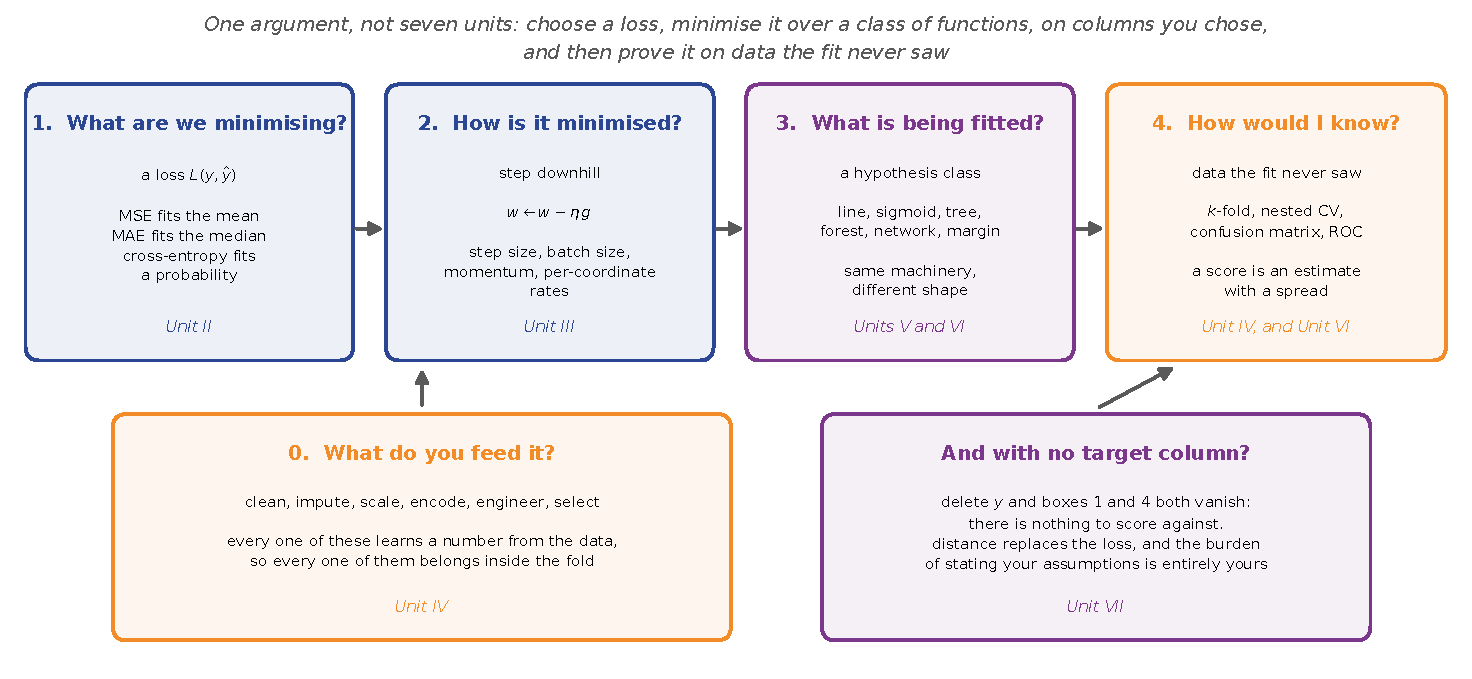
\includegraphics[width=\textwidth]{spine.pdf}
  \caption{The course on one page. Read left to right along the top: choose a
  loss, minimise it, over a class of functions, and then prove it on data the
  fit never saw. The bottom-left box feeds all four. The bottom-right box is
  what happens when the target column is deleted.}
  \label{fig:spine}
\end{figure}

\subsection{Unit II --- what quantity are we minimising}

A loss is not a scoring rule applied after the fact. It is the specification
of what the model will become. The demonstration that makes this concrete
took six sensor readings, corrupted one of them, and asked for the single
constant that best summarises them. Under squared error the answer moved from
$12.33$ to $25.67$ --- past every clean observation --- while under absolute
error it did not move at all. The reason is a one-line calculus fact: the
constant minimising $\sum (y_i - c)^2$ is the \emph{mean}, and the constant
minimising $\sum |y_i - c|$ is the \emph{median}.

\begin{keyidea}
Choosing a loss is choosing what the model becomes, not how it is graded.
Every property you later complain about --- sensitivity to outliers, refusal
to output a probability, indifference to a rare class --- was decided here.
\end{keyidea}

\subsection{Unit III --- how the minimisation is carried out}

Given a loss, descent is three questions: how big a step, computed from how
much data, and with how much memory of the last step. Those are the learning
rate, the batch size and the momentum coefficient. The payoff of having
separated Units II and III is that \emph{the answer does not depend on which
loss you picked}: the same gradient-descent loop fits a squared-error line, a
cross-entropy classifier and a ten-thousand-parameter network.

Two measurements from that unit are worth keeping. There is a hard stability
cliff: on one quadratic, $\eta = 1.00$ made the iterates cycle
$0 \to 6 \to 0$ forever and $\eta = 1.05$ sent them to $-17.18$ in twenty
steps. And the adaptive optimisers, tuned, all land within two per cent of
each other; what they really buy is a \emph{wider target} --- Adagrad worked
over $2.24$ decades of learning rate against plain SGD's $1.31$.

\subsection{Unit IV --- what you feed the optimiser}

This is the unit that decides your ceiling. One engineered product column took
a linear model from cross-validated $R^2 = 0.9065$ to $0.9978$; a random
forest reached the same place unaided, which is the useful form of the lesson
--- \emph{feature engineering is worth most to the simplest models}.

The rule that runs through the entire unit, and that Section~\ref{sec:mistakes}
prices, is one sentence.

\begin{keyidea}
Anything you learn from the data --- a mean, a median, a category list, a
rotation, a feature subset, a resampled row, a hyper-parameter --- is part of
the model, and belongs inside the cross-validation fold.
\end{keyidea}

\subsection{Units V and VI --- the same machinery, different classes}

Table~\ref{tab:zootab} is the point of these two units. Read it down the
columns rather than across the rows: the rows differ in $\mathcal{H}$ and in
$L$, and in almost nothing else.

\begin{table}[t]
  \centering \small
  \begin{tabular}{@{}llll@{}}
    \toprule
    \textbf{Method} & \textbf{Hypothesis class $\mathcal{H}$} &
      \textbf{Loss $L$} & \textbf{Minimised by} \\
    \midrule
    Least squares  & linear in $x$           & squared error       & closed form, $(X^\top X)^{-1}X^\top y$ \\
    Ridge, lasso   & linear in $x$           & squared $+$ $\Omega$ & closed form; coordinate descent \\
    Logistic       & linear in the log-odds  & cross-entropy       & gradient descent, Newton/IRLS \\
    Naive Bayes    & product of conditionals & (counting)          & closed-form counts \\
    Decision tree  & axis-aligned boxes      & impurity reduction  & greedy recursive search \\
    Random forest  & average of trees        & impurity reduction  & greedy $+$ bootstrap $+$ column sampling \\
    Boosting       & additive sum of trees   & any differentiable  & stagewise gradient steps \\
    Neural network & composed affine + nonlinearity & any differentiable & backpropagation and SGD \\
    SVM            & linear in a feature map & hinge $+ \lVert w \rVert^2$ & convex quadratic programme \\
    $k$-NN         & the training table itself & ---               & --- (there is no fit) \\
    \bottomrule
  \end{tabular}
  \caption{Nine supervised methods as three choices each. The differences
  between rows are real and they matter, but they are differences
  \emph{within one template}, not between unrelated inventions.}
  \label{tab:zootab}
\end{table}

Three connections in that table are worth stating explicitly, because they are
the ones examinations ask about.

\begin{itemize}[leftmargin=*]
  \item \textbf{Least squares is not an arbitrary choice.} Assume Gaussian
    noise, write the likelihood, take logarithms, and the log-likelihood is a
    constant minus $\mathrm{SSE}/(2\sigma^2)$. Maximising the likelihood
    \emph{is} minimising the sum of squared errors. Change the noise to
    Laplace and the maximum-likelihood estimator becomes least absolute
    deviations.
  \item \textbf{Logistic regression is least squares' template with two
    substitutions.} $\mathcal{H}$ becomes linear in the log-odds rather than
    in $y$, and $L$ becomes the Bernoulli negative log-likelihood. The
    gradient is then almost embarrassingly familiar:
    $\nabla L = X^\top(p - y)$, prediction minus truth, exactly as in the
    linear case.
  \item \textbf{An ensemble is not a better model; it is a bet on
    disagreement.} Bagging perturbs rows, forests additionally perturb
    columns, boosting changes the problem after each round. As the members
    become more correlated the benefit collapses; independence is the whole
    game.
\end{itemize}

\subsection{Unit VII --- what changes when there is no target}

Delete the $y$ column from equation~\eqref{eq:template} and two of its four
choices lose their meaning. There is no $L(y_i, f(x_i))$ because there is no
$y_i$; and there is no held-out score because there is nothing to be right
about. What replaces the loss is a \textbf{distance}, chosen by you; what
replaces the score is an \textbf{assumption}, stated by you.

That is not a gap in the theory. It is the defining property of the subject:
clustering \emph{proposes} a structure rather than discovering a fact, and the
proposal is a joint consequence of the data, the distance, the algorithm and
the settings. The measured consequence is stark. On \texttt{wine},
$k$-means agrees with the cultivar at ARI $0.3711$ on the raw columns and
$0.8975$ after standardising, because one column carries $99.77\%$ of the raw
variance and Euclidean distance is therefore almost entirely a comparison of
that one column. Nothing about the algorithm changed.

\begin{caution}[The commonest Unit VII error in scripts]
``The clustering was wrong because it did not match the labels.'' If you have
labels, you are not clustering. On \texttt{iris}, two internal criteria agree
on $k = 2$ and the species say $k = 3$; both are correct answers to different
questions. The number of clusters in the data and the number of classes in
the label column are different quantities.
\end{caution}

% =========================================================================
\section{The revision map}
\label{sec:map}

This section is deliberately short, and it is short on purpose. A revision
list that includes everything is worth nothing, because it cannot help you
allocate an evening. What follows is what is \emph{genuinely} examinable:
calculations you can be asked to produce with a pen, and derivations you can
be asked to reproduce. Everything else you should be able to recognise and
discuss, which is a much lower bar.

\begin{table}[t]
  \centering \small
  \begin{tabular}{@{}p{1.1cm}p{4.4cm}p{8.3cm}@{}}
    \toprule
    \textbf{Unit} & \textbf{The one idea} & \textbf{What you can be asked to
      compute or derive} \\
    \midrule
    I &
    Learning is fitting a function from examples; three kinds of task &
    classifying a described problem as supervised, unsupervised or
    reinforcement; MAE, MSE and RMSE on a handful of numbers; a 1-NN
    prediction from a distance table \\[0.35em]
    II &
    Choosing a loss chooses what the model becomes &
    minimising a loss over a constant and showing MSE gives the mean and MAE
    the median; writing cross-entropy for a Bernoulli label; explaining why a
    squared error is not robust \\[0.35em]
    III &
    Step downhill: how big, from how much data, with how much memory &
    one gradient-descent step by hand on a quadratic; the divergence
    condition on $\eta$; one momentum update and one Adam update including
    the bias correction \\[0.35em]
    IV &
    What you feed it decides what it can find &
    the survival probability $(1-p)^d$ under listwise deletion; the $z$, IQR
    and modified-$z$ outlier rules on a small column; one standardisation by
    hand; deciding what must sit inside the fold, and saying why \\[0.35em]
    V &
    Least squares has an answer you can write down, and one dial controls it
    &
    $b_1 = S_{xy}/S_{xx}$, $b_0 = \bar y - b_1 \bar x$, SSE and $R^2$; the
    normal equations on a $2\times2$ or $3\times3$; the Gaussian-MLE
    derivation; ridge $\hat\beta = (X^\top X + \lambda I)^{-1} X^\top y$ and
    the invertibility argument; soft thresholding \\[0.35em]
    VI &
    One recipe, several hypothesis classes &
    entropy, information gain and gain ratio on a small table; a $k$-NN
    prediction and the effect of $k$; Bayes with a prior, and naive Bayes
    with Laplace smoothing; one AdaBoost round ($\varepsilon$, $\alpha$,
    reweighting); one forward and backward pass on a small network; the
    margin and $\alpha_i$ on a few separable points; a confusion matrix,
    precision, recall, $F_1$, and a ROC point with its AUC \\[0.35em]
    VII &
    Delete the target and the distance becomes the whole decision &
    building a proximity matrix; a complete agglomerative run under single
    and under complete linkage, matrix rewritten after every merge; one
    Lloyd iteration of $k$-means; the silhouette of one point; deciding
    whether a described dissimilarity is a metric \\
    \bottomrule
  \end{tabular}
  \caption{The revision map. If a topic is not in the right-hand column it is
  still on the syllabus --- but it will be tested by asking you to explain,
  not to compute.}
  \label{tab:map}
\end{table}

\paragraph{Which notes to reread, and in what order.} If you have one evening:
the notes on \emph{loss functions} for the mean-versus-median demonstration,
the notes on \emph{cross-validation and model selection} for what belongs
inside the fold, the notes on \emph{decision trees} for entropy and gain, the
notes on \emph{neural networks} for the backward pass, and the notes on
\emph{classification evaluation} for the ROC staircase. Those five carry most
of the computable marks in the course. If you have a week, add the
\emph{regularization} notes for the ridge invertibility proof and soft
thresholding, the \emph{Bayesian} notes for the base-rate inversion, and the
\emph{hierarchical clustering} notes for the two linkage runs.

\paragraph{What is not worth memorising.} Library argument names. Coefficient
tables you can look up. Any number you can recompute in ten seconds. Spend
the time instead on the arithmetic in Section~\ref{sec:hand}, all of which you
can be asked to \emph{produce}.

% =========================================================================
\section{One dataset, every model}
\label{sec:zoo}

The most useful revision exercise in the whole course is also the simplest:
take one dataset and run everything on it under one protocol. It settles, with
numbers, a question that folklore gets wrong.

\subsection{The protocol}

\begin{lstlisting}
X, y = load_breast_cancer(return_X_y=True)     # 569 x 30, 357 benign
cv = RepeatedStratifiedKFold(n_splits=5, n_repeats=4, random_state=24)

for name, est in seven_models.items():
    for tr, te in cv.split(X, y):
        pipe = Pipeline([("sc", StandardScaler()), ("m", clone(est))])
        pipe.fit(X[tr], y[tr])                 # scaler refitted every fold
        acc.append(accuracy_score(y[te], pipe.predict(X[te])))
        auc.append(roc_auc_score(y[te], score_of(pipe, X[te])))
\end{lstlisting}

Two choices in those six lines are the difference between a measurement and an
anecdote. \emph{Twenty} folds rather than five, so that the fold-to-fold
spread is itself estimated. And the scaler \emph{inside} the pipeline, so that
the mean and standard deviation used to transform a validation row were
computed without ever looking at it.

\subsection{What it produced}

\begin{codeout}
X shape (569, 30)   positives 357   negatives 212   majority rate 0.6274
folds = 20

model                    acc      sd     AUC      sd   fit ms  pred ms
LogisticRegression    0.9767  0.0096  0.9943  0.0059      2.3     0.24
KNN (k=11)            0.9675  0.0179  0.9898  0.0077      0.6     1.39
DecisionTree          0.9324  0.0191  0.9290  0.0198      6.1     0.35
RandomForest          0.9626  0.0163  0.9899  0.0073    341.3     7.08
GradientBoosting      0.9605  0.0212  0.9908  0.0085    366.9     0.62
MLP (100,)            0.9767  0.0122  0.9939  0.0067    225.9     0.44
SVM (RBF)             0.9745  0.0099  0.9956  0.0046      2.5     0.71
\end{codeout}

\begin{caution}[Two of those nine columns are measurements, not results]
The accuracies, the standard deviations and the AUCs above reproduce exactly:
fixed data, one seed, same answer on your machine as on mine. \textbf{The two
millisecond columns do not.} They depend on your processor, your BLAS build
and what else is running, and repeated runs of this identical script moved
the MLP's fit time between $225$ and $253$ milliseconds without a line of
code changing.

So the seconds are reported here as one measurement and are never the basis
of a claim. When this lecture says a model is expensive, it says so in
something countable --- how many parameters were fitted, how many trees, how
many support vectors --- and those are the same everywhere:

\begin{codeout}
  model                           fitted quantities
  LogisticRegression                31 coefficients
  KNN (k=11)           0 fitted, 13650 numbers stored
  DecisionTree                             31 nodes
  RandomForest               300 trees, 10534 nodes
  GradientBoosting            100 trees, 1406 nodes
  MLP (100,)                3201 weights and biases
  SVM (RBF)                     106 support vectors
\end{codeout}

That table explains the millisecond column without depending on any machine.
The MLP fits $3201$ weights against logistic regression's $31$ --- a factor of
$\mathbf{103}$, exactly --- for two accuracies that agree to four decimal
places. $k$-NN fits nothing at all and stores $13{,}650$ numbers, which is why
it is the cheapest to fit and the dearest to predict.
\end{caution}

Six of the seven sit inside a band of $0.017$ in accuracy. The seventh, the
single unpruned tree, is the only one clearly worse --- and it is also the
only model in the list with no averaging, no penalty and no margin anywhere
in it. A majority-class baseline would have scored $0.6274$, so
\textbf{the distance from any real model to the baseline is roughly twenty
times the distance between the real models}.

\begin{figure}[t]
  \centering
  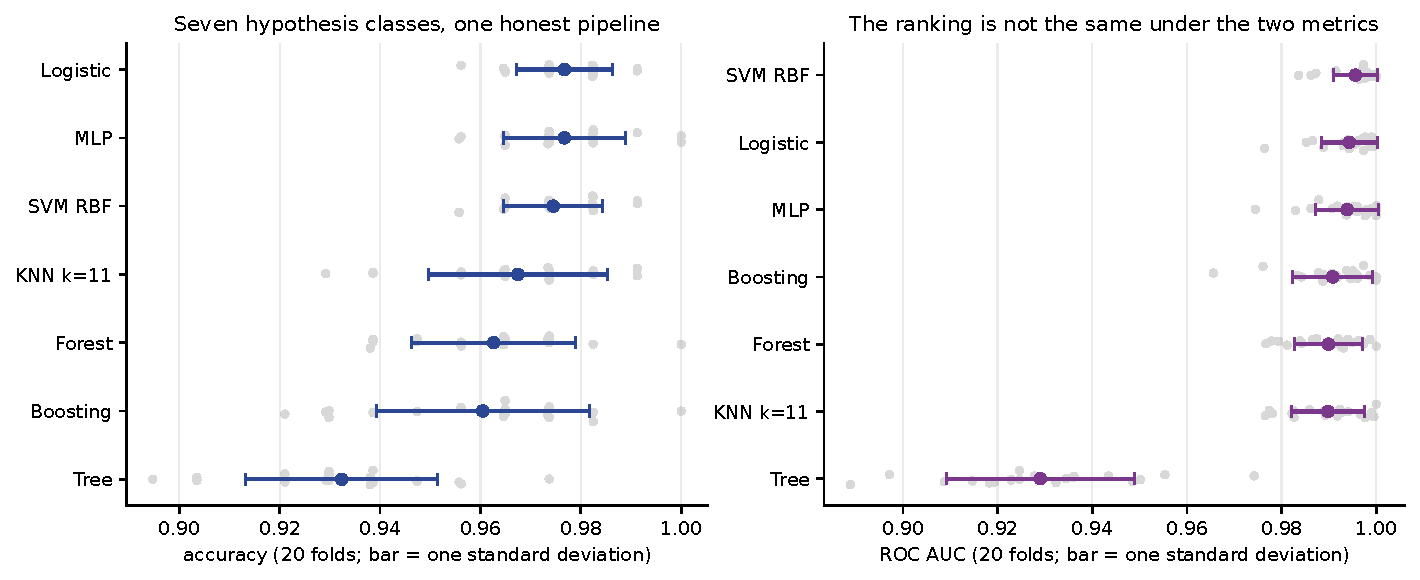
\includegraphics[width=\textwidth]{allmodels.pdf}
  \caption{Seven hypothesis classes on 569 patients, twenty folds each. The
  grey dots are individual folds; the bars are one standard deviation. Left,
  accuracy; right, ROC AUC. Note that the order is not the same in the two
  panels.}
  \label{fig:allmodels}
\end{figure}

\subsection{Is the winner the winner?}

\begin{codeout}
best by AUC      : SVM (RBF) 0.9956
second by AUC    : LogisticRegression 0.9943
gap              : 0.0013
fold-to-fold sd  : 0.0046 (winner)  0.0059 (runner-up)
paired t-test    : t = 2.4697   p = 0.0232
folds the nominal winner LOST : 6 of 20
\end{codeout}

The paired test is significant at the conventional level and the result is
\emph{immaterial}. A gap of $0.0013$ against a fold-to-fold spread of
$0.0046$ is a quarter of the noise; the nominal winner lost six folds out of
twenty. On accuracy the same two models go the other way by $+0.0022$, with
$p = 0.3965$, seven wins, four losses and \textbf{nine ties}.

\begin{keyidea}
A difference smaller than the fold-to-fold spread is not a difference. Report
the spread every time you report a score, and when the intervals overlap,
choose on cost, interpretability or maintainability instead --- because those
you can actually measure.
\end{keyidea}

\begin{figure}[t]
  \centering
  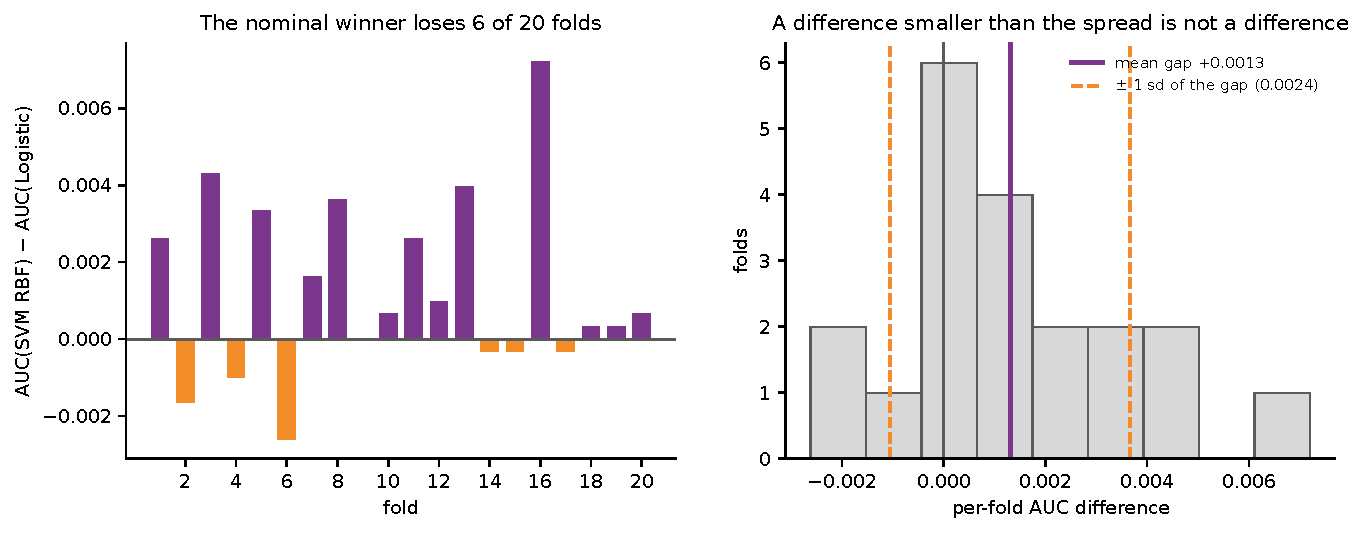
\includegraphics[width=0.92\textwidth]{spread.pdf}
  \caption{Left: the per-fold AUC difference between the two best models. Six
  bars point the wrong way. Right: the same twenty differences as a
  histogram, with the mean gap and one standard deviation of the gap marked.
  The distribution straddles zero comfortably.}
  \label{fig:spread}
\end{figure}

\subsection{The rank depends on the metric}

\begin{codeout}
rank  by accuracy           by AUC
1     LogisticRegression    SVM (RBF)
2     MLP (100,)            LogisticRegression
3     SVM (RBF)             MLP (100,)
4     KNN (k=11)            GradientBoosting
5     RandomForest          RandomForest
6     GradientBoosting      KNN (k=11)
7     DecisionTree          DecisionTree
models whose rank changes with the metric : 5 of 7
\end{codeout}

Five of seven change place. Accuracy and AUC are answering different
questions: accuracy grades one threshold, AUC grades the whole ranking. Both
are legitimate; neither is ``the'' score. Name the metric before you name the
winner, and choose the metric from the problem.

\subsection{And what the seven cost}

\begin{figure}[t]
  \centering
  
\includegraphics[width=0.80\textwidth]{cost.pdf}
  \caption{Fit and predict time per fold, log scale --- a measurement on one
  machine, not a property of the algorithms. The countable version: gradient
  boosting fits $100$ trees and $1406$ nodes and scores no better than
  logistic regression's $31$ coefficients. $k$-NN is the mirror image ---
  nothing fitted at all, and the highest predict cost of the seven, because
  it does all its work at predict time.}
  \label{fig:cost}
\end{figure}

\begin{tryit}
Rerun the protocol with \texttt{load\_wine} in place of
\texttt{load\_breast\_cancer} and with \texttt{n\_repeats=10}. Two things
should happen: every standard deviation grows, because wine has 178 rows and
each fold holds only 36; and the ordering of the middle five models shuffles.
If your conclusion changes when you change the seed, you did not have a
conclusion.
\end{tryit}

% =========================================================================
\section{Choosing a method, and defending the choice}
\label{sec:choose}

Section~\ref{sec:zoo} showed that on a clean, well-separated, moderately sized
table the choice of model barely matters. That is the common case and it is
worth knowing. This section is about the uncommon cases, where the choice
matters enormously --- and every row of Table~\ref{tab:choose} is grounded in
a measurement rather than in received wisdom.

\begin{figure}[t]
  \centering
  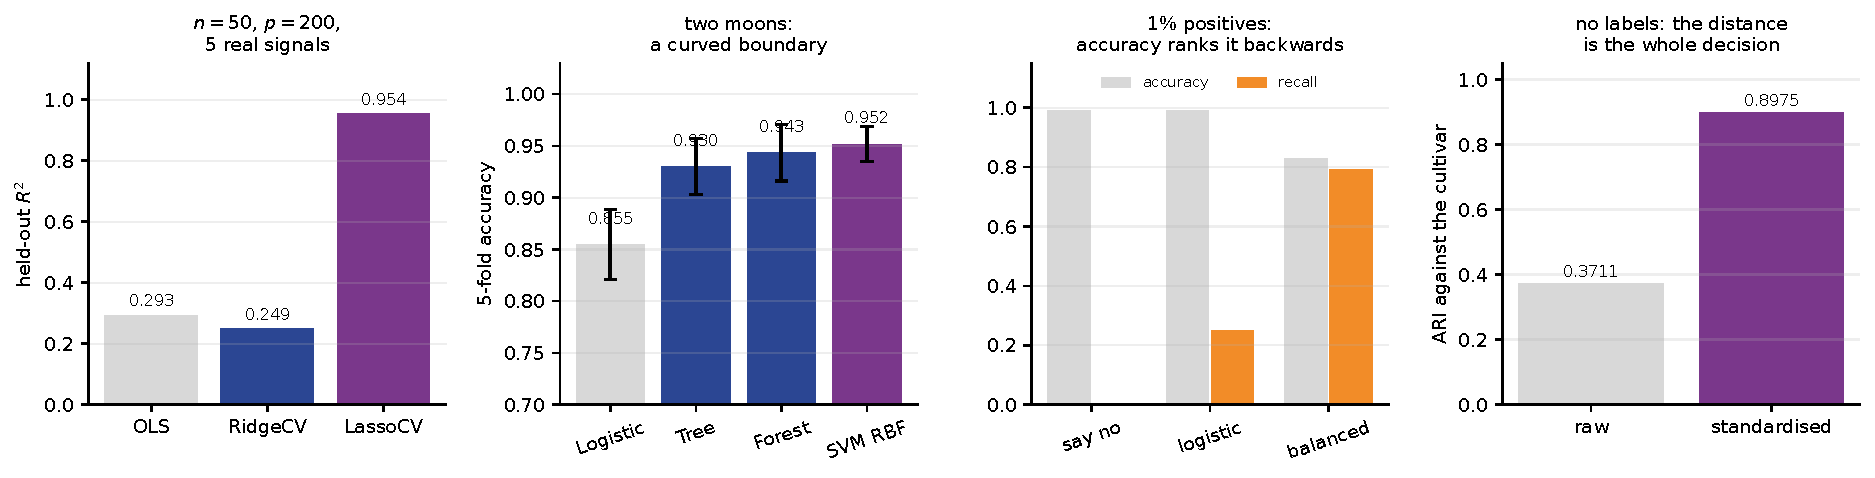
\includegraphics[width=\textwidth]{regimes.pdf}
  \caption{Four regimes in which the models are not interchangeable. Left to
  right: a sparse truth with more columns than rows; a curved decision
  boundary; one per cent positives; and no labels at all.}
  \label{fig:regimes}
\end{figure}

\begin{table}[t]
  \centering \small
  \begin{tabular}{@{}p{2.7cm}p{3.1cm}p{8.0cm}@{}}
    \toprule
    \textbf{Situation} & \textbf{Try first} & \textbf{The measurement behind
      the advice} \\
    \midrule
    Few rows, many
    columns, and you
    believe the truth is
    sparse &
    lasso; elastic net if
    the columns are
    correlated &
    $n = 50$, $p = 200$, five real signals: OLS test $R^2 = +0.2926$,
    cross-validated ridge $+0.2492$, cross-validated lasso
    $\mathbf{+0.9543}$ --- and the lasso kept \textbf{5 of the 5} real
    columns. Ridge cannot help here because it never returns a zero \\[0.4em]
    You must explain the
    model to someone &
    penalised logistic
    regression, or a
    shallow tree &
    on \texttt{breast\_cancer}, thirty readable coefficients score AUC
    $0.9947 \pm 0.0042$ against gradient boosting's $0.9919 \pm 0.0059$. The
    readable model cost \textbf{nothing at all} --- it was marginally ahead
    \\[0.4em]
    The boundary is
    clearly non-convex &
    RBF SVM, $k$-NN, or
    a forest &
    two moons, 5-fold accuracy: logistic $0.8550$, tree $0.9300$, forest
    $0.9433$, $k$-NN $0.9500$, SVM $\mathbf{0.9517}$. The linear model is
    nine points behind and no amount of tuning closes it \\[0.4em]
    Heavy class
    imbalance &
    any model --- but
    change the metric and
    the threshold &
    at $1\%$ positives, always-say-no scores accuracy $0.9900$; the model
    that finds 19 of 24 positives scores $0.8275$. Average precision
    baseline is the prevalence, $0.0100$, not $0.5$ \\[0.4em]
    No labels at all &
    $k$-means or DBSCAN,
    after deciding the
    distance &
    $k$-means on \texttt{wine}: ARI $0.3711$ raw, $\mathbf{0.8975}$
    standardised. One column carried $99.77\%$ of the raw variance. The
    pre-processing decision was worth more than the algorithm \\[0.4em]
    Very many rows, and
    latency matters &
    a linear model; a
    forest if you can
    wait &
    40{,}000 rows: logistic fits in $\mathbf{0.04}$ s and predicts in under
    $0.01$ s; the forest fits in $10.86$ s; the SVM fits in $5.32$ s and
    takes $2.54$ s to predict 10{,}000 rows \\
    \bottomrule
  \end{tabular}
  \caption{The choosing table. Each row names a property of the
  \emph{problem}, not a preference.}
  \label{tab:choose}
\end{table}

\begin{worked}[Reading the first row properly]
The sparse-truth row is the one students most often get backwards, so it is
worth spelling out. There were $200$ columns and $50$ rows, so ordinary least
squares is already under-determined: \texttt{LinearRegression} returns the
minimum-norm solution, which is ridge in the limit $\lambda \to 0$. That
solution reached test $R^2 = +0.2926$. Cross-validated ridge chose the
smallest $\alpha$ in its grid and did essentially the same thing,
$+0.2492$. Cross-validated lasso reached $+0.9543$ and kept 31 columns, five
of which were the five real ones.

Ridge did not fail because ridge is worse. It failed because the truth was
\emph{sparse} and ridge cannot express sparsity --- on a swept path its
smallest coefficient anywhere was $1.455 \times 10^{-3}$, never zero. Reverse
the experiment, with a dense truth and correlated columns, and ridge wins
instead. Neither penalty dominates, which is exactly why both are on the
syllabus.
\end{worked}

\begin{caution}[Two answers that are always wrong]
\textbf{``I tried them all and picked the best score.''} That is a
hyper-parameter search with the evaluation set as its objective, and
Section~\ref{sec:mistakes} prices it at $+0.0515$ on pure noise, wrong on 17
of 20 trials.

\textbf{``A neural network, because it is the most powerful.''} On these 569
patients the MLP scored $0.9767$ and logistic regression scored $0.9767$ ---
identical to four decimals --- and the MLP fitted $3201$ weights against
logistic regression's $31$, exactly $103\times$ as many.
Capacity you do not need is capacity you have to regularise, tune and defend.
\end{caution}

\subsection{How to phrase a defensible choice}

A good answer has three parts, in this order.

\begin{enumerate}[leftmargin=*]
  \item \textbf{A property of the problem.} ``There are 80 rows and 12{,}000
    columns, and the clinician needs a short list of genes.''
  \item \textbf{The family that property implies, with the mechanism.}
    ``Lasso, because the $L_1$ penalty has a corner at zero and therefore
    returns exact zeros; ridge shrinks but never deletes.''
  \item \textbf{What would refute it.} ``If the true signal is dense rather
    than sparse --- many small effects --- the lasso will delete real
    predictors and ridge will beat it. I would check by comparing
    cross-validated scores for both, and by looking at how stable the
    selected set is across bootstrap resamples.''
\end{enumerate}

The third part is the one almost everybody omits, and it is the one that
distinguishes a student who has understood the course.

% =========================================================================
\section{The five mistakes that cost the most}
\label{sec:mistakes}

These five are ranked by what they actually cost, in marks and in accuracy.
Four of them are score inflations and can be drawn on one axis
(Figure~\ref{fig:mistakes}); the fifth is not a score at all.

\begin{figure}[t]
  \centering
  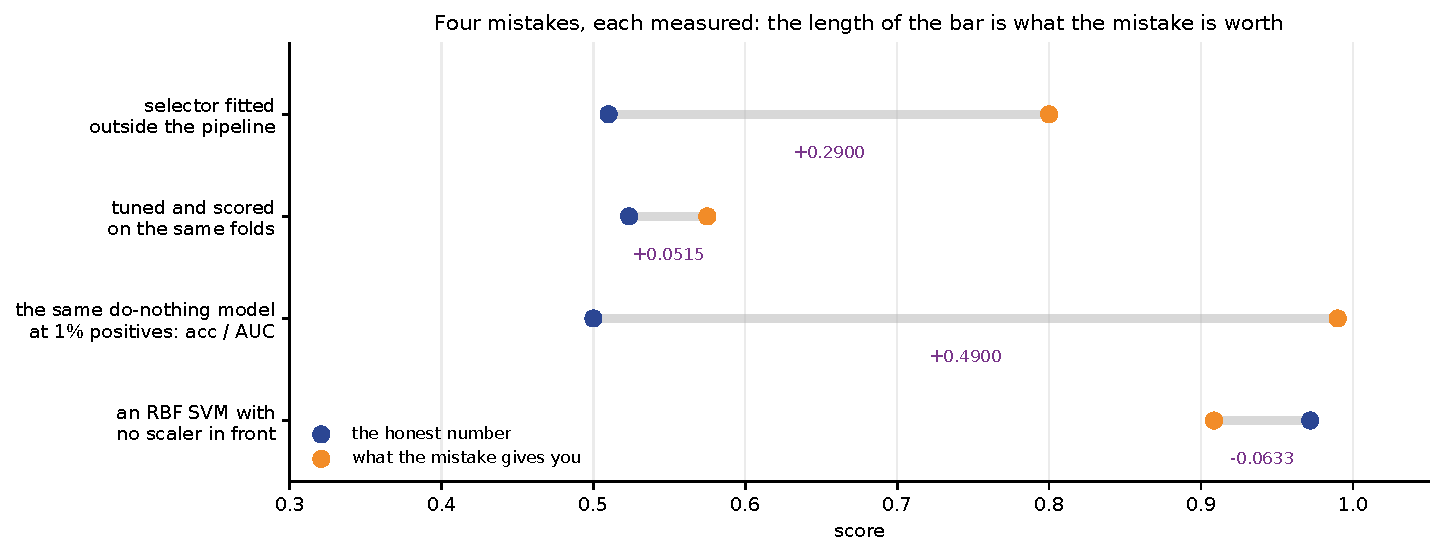
\includegraphics[width=0.94\textwidth]{mistakes.pdf}
  \caption{Four mistakes with their measured price. Orange is the number the
  mistake produces; blue is the honest number. The fourth row runs the other
  way: forgetting the scaler \emph{costs} you $0.0633$ rather than inflating
  anything.}
  \label{fig:mistakes}
\end{figure}

\subsection{Mistake 1: fitting a transformer outside the pipeline}
\label{sec:m1}

\begin{lstlisting}
rng = np.random.default_rng(24)
X = rng.normal(size=(100, 500))     # 500 columns of pure noise
y = rng.integers(0, 2, size=100)    # coin-flip labels: the truth is 0.5

sel   = SelectKBest(f_classif, k=10).fit(X, y)      # <-- sees every row
wrong = cross_val_score(LogisticRegression(max_iter=5000),
                        sel.transform(X), y, cv=cv)

right = cross_val_score(Pipeline([("k", SelectKBest(f_classif, k=10)),
                                  ("m", LogisticRegression(max_iter=5000))]),
                        X, y, cv=cv)

for r in range(20):                    # a sweep: 20 FRESH noise problems,
    rg = np.random.default_rng(1000 + r)   # one stream, twenty draws
    ...                                # the spread across them is the result
\end{lstlisting}
\begin{codeout}
500 pure-noise columns, coin-flip labels; truth is 0.5000
selection outside the pipeline   0.8000
selection inside the pipeline    0.5100
overstatement                    +0.2900
over 20 fresh noise problems: leaky 0.7535, honest 0.5000
the leaky protocol scored higher on 20 of 20
\end{codeout}

There is no signal in that data at all. The labels are coin flips. And the
leaky protocol reports an accuracy of $0.80$, with a straight face, on
\emph{twenty out of twenty} fresh problems.

The mechanism is worth saying out loud, because once you have said it you will
never make the mistake again. \texttt{SelectKBest} was shown the labels of
every row, including the rows that later became the validation fold. Among
500 coin-flip columns, ten will look predictive by chance --- and once those
ten have been chosen \emph{using the answers}, the validation fold is no
longer unseen. The cross-validation that follows is measuring how well a
model fits noise it was pointed at.

\begin{caution}
The same error wears several costumes, and the course measured all of them:
scaling before the split, $+0.0034$; imputing before the split, nothing
measurable; deciding which rows to drop before the split, $+0.1702$ of $R^2$;
oversampling before the split, $F_1 = 0.8942$ against an honest $0.1133$,
because $100\%$ of the minority test rows were byte-identical copies of
training rows. The size of the damage varies enormously. The rule does not.
\end{caution}

\subsection{Mistake 2: tuning and evaluating on the same folds}
\label{sec:m2}

\begin{lstlisting}
gs = GridSearchCV(pipe, grid_of_22_models, cv=inner).fit(X, y)
print(gs.best_score_)               # a MAXIMUM over 22 noisy estimates

nested = cross_val_score(GridSearchCV(pipe, grid_of_22_models, cv=inner),
                         X, y, cv=outer)   # an ESTIMATE of generalisation
\end{lstlisting}
\begin{codeout}
the grid is 22 model-and-setting combinations
breast_cancer   best_score_ 0.9824   nested 0.9824 +/- 0.0125
                optimism    -0.0000
100x30 pure noise, coin-flip labels, 20 trials; truth 0.5000
  best_score_ 0.5750   nested 0.5235   optimism +0.0515
  best_score_ exceeded the nested estimate on 17 of 20
\end{codeout}

Report both halves of that, because both are instructive. On
\texttt{breast\_cancer} --- an easy, well-separated, 569-row problem --- the
optimism was \textbf{zero to four decimal places}. On 100 rows of pure noise
the same grid reported $0.5750$ where the truth is $0.5000$.

\begin{keyidea}
\texttt{best\_score\_} is the maximum of a set of noisy estimates, and the
maximum of noisy estimates is biased upwards. How badly depends on how many
combinations you tried and how noisy each estimate was --- and you cannot
tell which regime you are in \emph{without} the nested loop. That is the
argument for always running it.
\end{keyidea}

\subsection{Mistake 3: quoting accuracy under imbalance}
\label{sec:m3}

\begin{codeout}
test prevalence 0.0100, 24 positives in 2400 rows
model                           acc      AUC       AP   recall
always say no                0.9900   0.5000   0.0100   0.0000
logistic, default            0.9917   0.9084   0.4690   0.2500
logistic, class_weight       0.8275   0.8938   0.3035   0.7917
the balanced model finds 19 of the 24 positives; accuracy ranks it LAST
\end{codeout}

Read the last row twice. The only model in the table that actually
\emph{finds} the rare class --- nineteen of the twenty-four positives ---
scores $0.8275$, and accuracy therefore ranks it behind a model that has
never predicted a positive in its life. If accuracy is your objective, the
optimal policy at one per cent prevalence is to do nothing.

\begin{figure}[t]
  \centering
  
\includegraphics[width=0.85\textwidth]{imbalance.pdf}
  \caption{One model, one set of scores, one test set. ROC AUC is invariant
  to the class balance and looks excellent. Average precision, whose baseline
  is the prevalence rather than $0.5$, is the honest summary at this
  prevalence.}
  \label{fig:imbalance}
\end{figure}

\begin{caution}
Quote the confusion matrix, recall and precision at a stated threshold, and
average precision with its baseline. If you quote a single number for an
imbalanced problem, quote average precision and say what the prevalence was
--- ``AP $0.4690$ against a baseline of $0.0100$'' is informative;
``$99.2\%$ accurate'' is not.
\end{caution}

\subsection{Mistake 4: unscaled distance-based or gradient-based methods}
\label{sec:m4}

\begin{codeout}
model                     raw   scaled     gain
KNN (k=11)             0.9401   0.9683  +0.0282
SVM (RBF)              0.9086   0.9719  +0.0633
MLP (100,)             0.9244   0.9754  +0.0510
LogisticRegression     0.9543   0.9771  +0.0229
DecisionTree           0.9368   0.9368  +0.0000
RandomForest           0.9560   0.9560  +0.0000
\end{codeout}

The two zeros are exact, not rounded. A tree splits on $x_j < t$, and that
predicate is unchanged by any strictly increasing transformation of $x_j$ ---
so the tree is the same tree, node for node, and its predictions are
identical. Everything that computes a distance, an inner product or a
gradient sees a completely different problem.

\begin{worked}[Why $k$-NN in particular collapses]
Take two \texttt{breast\_cancer} patients and decompose the squared Euclidean
distance between them column by column. The widest column supplies
$\mathbf{0.904482}$ of it, and the twenty-seven narrowest columns share
$0.007655$ between them. Unscaled $k$-NN on that table is not a
thirty-feature classifier; it is a one-feature classifier with twenty-nine
decorations. That is the whole of the $+0.0282$.
\end{worked}

\begin{figure}[t]
  \centering
  
\includegraphics[width=\textwidth]{scaling.pdf}
  \caption{Left, the six models with and without a scaler in the pipeline;
  the two tree-based rows are exactly unchanged. Right, the column-by-column
  decomposition of the squared distance between two unscaled patients.}
  \label{fig:scaling}
\end{figure}

\subsection{Mistake 5: reading a coefficient as a cause}
\label{sec:m5}

\begin{codeout}
diabetes, total serum cholesterol (s1)
  fitted on its own            +0.4723
  with the other nine present  -1.0900
  the sign flips and the magnitude grows x2.31
  predictors that change sign this way: 4 of 10 -- age, sex, s1, s3
\end{codeout}

Both numbers are correct. They answer different questions. $+0.4723$ is the
average difference in outcome between patients whose cholesterol differs by
one unit, \emph{averaged over everything else}. $-1.0900$ is the same
difference \emph{among patients matched on the other nine measurements}. Four
of the ten predictors change sign between the two.

To make the point without any ambiguity, build a problem where the truth is
known by construction:

\begin{lstlisting}
Z  = rng.normal(size=4000)                    # the confounder
X  = Z + rng.normal(scale=0.5, size=4000)     # X is caused by Z, and only Z
Y  = 3.0 * Z + rng.normal(scale=0.5, size=4000)   # X appears nowhere here
\end{lstlisting}
\begin{codeout}
a designed confounder: X <- Z -> Y, X does not enter Y at all
  slope of Y on X alone        +2.3662   (R^2 0.7790)
  slope of Y on X given Z      -0.0119
  true causal effect of X on Y +0.0000
\end{codeout}

A regression of $Y$ on $X$ reports a slope of $+2.3662$ and explains
$78\%$ of the variance. The causal effect of $X$ on $Y$ is exactly zero. No
amount of data, no better optimiser and no larger model will fix this,
because it is not a statistical error --- it is a question about the world
that the data cannot answer.

\begin{keyidea}
The defensible wording is: ``holding the other predictors in this model
fixed, a one-unit increase in $x_j$ is \emph{associated with} a change of
$b_j$ in the fitted mean of $y$.'' Not ``causes''. Not ``if we increase
$x_j$''. And never without naming which other predictors were in the model.
\end{keyidea}

\begin{figure}[t]
  \centering
  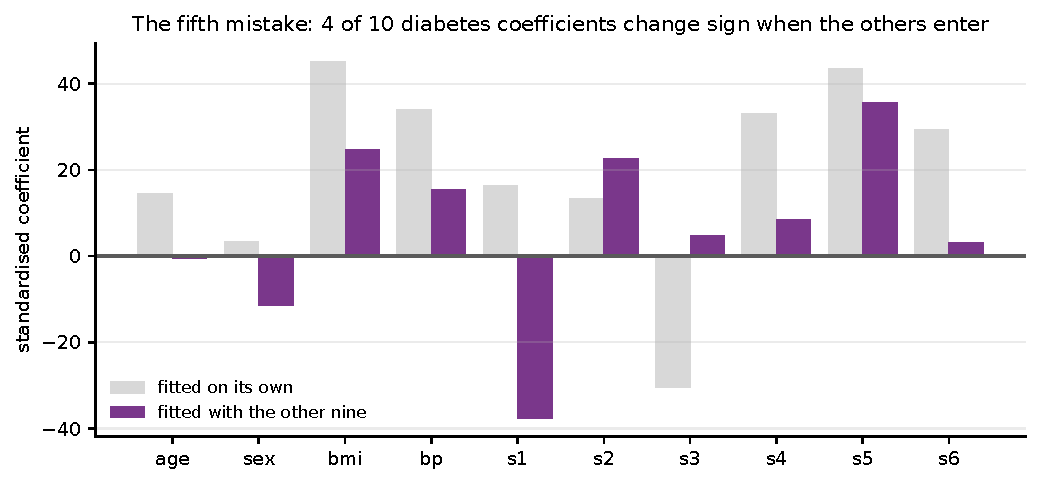
\includegraphics[width=0.85\textwidth]{coefsign.pdf}
  \caption{Standardised coefficients for the ten diabetes predictors, fitted
  one at a time and fitted together. Four change sign. Standardising cannot
  change a sign; it only makes the ten bars comparable.}
  \label{fig:coefsign}
\end{figure}

% =========================================================================
\section{End to end: raw arrays to a defended result}
\label{sec:e2e}

Everything above is a fragment. This section is one continuous run, in the
order you would really do it, on \texttt{breast\_cancer} with three per cent
of its cells deleted at random so that the imputer has work to do. The
positive class is \textbf{malignant}, which is the clinically sensible
framing and makes the cost asymmetry real.

\begin{figure}[t]
  \centering
  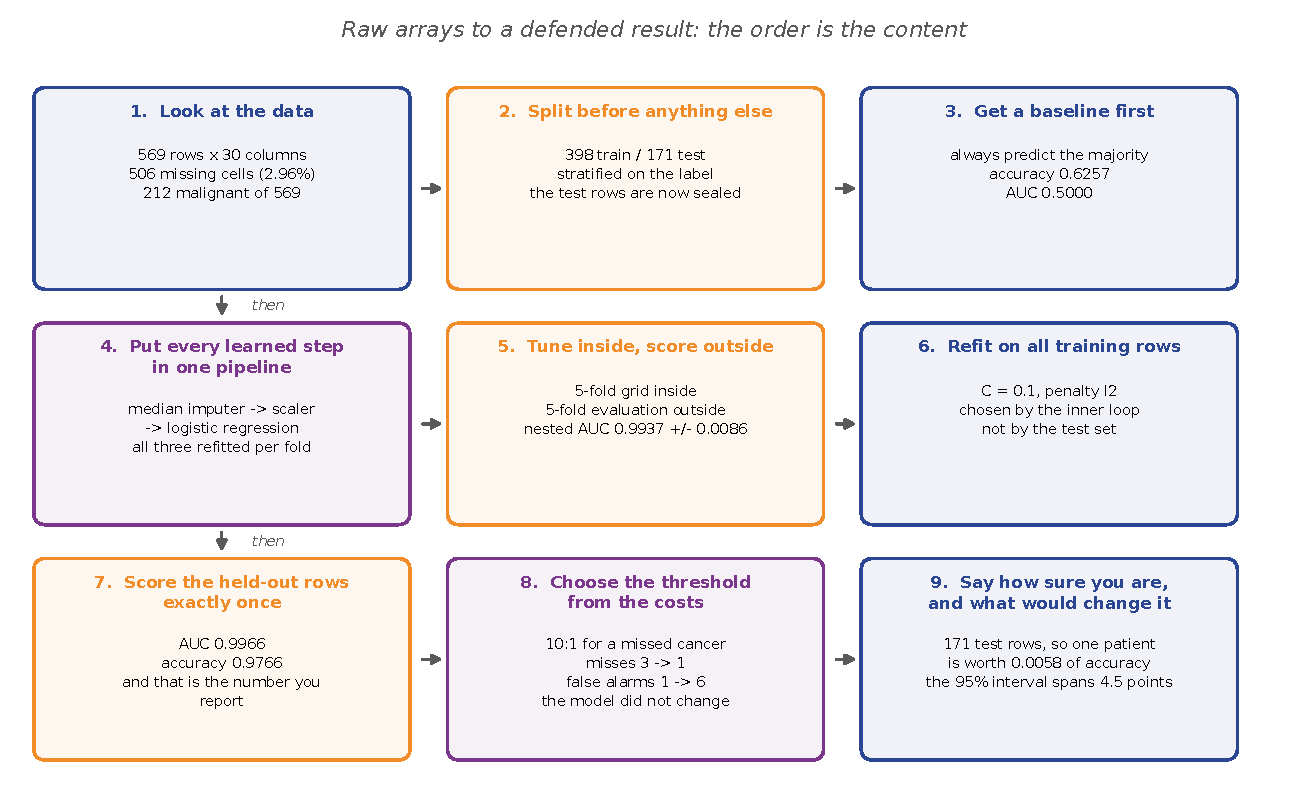
\includegraphics[width=\textwidth]{pipeline.pdf}
  \caption{The nine steps, with the measured result of each. The order is not
  a stylistic preference: steps 2 and 4 are what make step 7 meaningful.}
  \label{fig:pipeline}
\end{figure}

\subsection{Steps 0 to 3: look, split, baseline, one pipeline}

\begin{lstlisting}
X, y0 = load_breast_cancer(return_X_y=True)
y = 1 - y0                                  # positive = malignant
Xm = X.copy(); Xm[rng.random(X.shape) < 0.03] = np.nan

Xtr, Xte, ytr, yte = train_test_split(Xm, y, test_size=0.30,
                                      stratify=y, random_state=24)
base = DummyClassifier(strategy="most_frequent").fit(Xtr, ytr)

pipe = Pipeline([("imp", SimpleImputer(strategy="median")),
                 ("sc",  StandardScaler()),
                 ("m",   LogisticRegression(max_iter=5000,
                                            solver="liblinear"))])
\end{lstlisting}
\begin{codeout}
step 0  X (569, 30), 506 missing cells (2.96%), 229 complete rows of 569
        positive class = malignant, 212 of 569 rows (0.3726)
step 1  train 398, test 171, stratified (prevalence 0.3719 / 0.3743)
step 2  majority class: accuracy 0.6257, AUC 0.5000
step 3  imputer -> scaler -> model, all three refitted inside every fold
\end{codeout}

Look at step 0 again. Three per cent of the \emph{cells} are missing and only
$229$ of $569$ rows are complete: listwise deletion would throw away
$\mathbf{340}$ patients to remove $506$ numbers. That is $(1-p)^d$ with
$p = 0.03$ and $d = 30$, which is $0.40$, and the measured $229/569 = 0.402$.
The exponential in the number of columns is the reason imputation exists.

Step 2 is the step most often skipped. A baseline is not a formality: at
$0.6257$ it tells you immediately that any accuracy below about $0.63$ is
worse than doing nothing, and it gives the reader something to compare your
number against.

\subsection{Steps 4 to 6: tune inside, score outside, then score once}

\begin{lstlisting}
grid   = {"m__C": [0.001, 0.01, 0.1, 1, 10, 100], "m__penalty": ["l1", "l2"]}
inner  = StratifiedKFold(5, shuffle=True, random_state=24)
outer  = StratifiedKFold(5, shuffle=True, random_state=25)

nested = cross_val_score(GridSearchCV(pipe, grid, cv=inner,
                                      scoring="roc_auc"),
                         Xtr, ytr, cv=outer, scoring="roc_auc")
gs     = GridSearchCV(pipe, grid, cv=inner, scoring="roc_auc").fit(Xtr, ytr)
s      = gs.predict_proba(Xte)[:, 1]        # the test set, touched ONCE
\end{lstlisting}
\begin{codeout}
step 4  nested CV on the training rows: AUC 0.9937 +/- 0.0086
        (range 0.9787 .. 1.0000)
step 5  best params {'m__C': 0.1, 'm__penalty': 'l2'}, best_score_ 0.9941
        best_score_ - nested = +0.0004
step 6  held-out rows, scored once: AUC 0.9966, accuracy 0.9766
        confusion matrix  TN 106  FP 1  FN 3  TP 61
        recall 0.9531   precision 0.9839
\end{codeout}

The optimism at step 5 is $+0.0004$ --- negligible, because the grid has
twelve entries and the problem is easy. That is a result, not a licence to
skip the nested loop: you only know it is $+0.0004$ because you ran it.

\begin{caution}
The test set was touched exactly once, at step 6. If you look at a test score
and then change anything --- a hyper-parameter, a feature, a model --- it is
no longer a test set. It is a validation set, and you have no test set at
all. This is the discipline that makes the number in your report mean
something.
\end{caution}

\subsection{Step 7: the threshold is a separate decision}

\begin{codeout}
Youden J on the out-of-fold scores picks 0.4778 (J = 0.9502)
at 10:1 costs the out-of-fold minimum is at 0.2525

threshold           TN      FP      FN    recall  precision
0.5000 default     106       1       3    0.9531     0.9839
0.4778 Youden      106       1       3    0.9531     0.9839
0.2525 cost        101       6       1    0.9844     0.9130
\end{codeout}

Two things to notice, and one of them is a null result reported as it
happened. Youden's $J$, chosen honestly on out-of-fold training scores,
picked $0.4778$ and changed \textbf{nothing at all} on the test rows. That is
not a failure of the method: Youden is the equal-cost answer, the default
$0.5$ is close to it here, and on a well-separated problem there are simply no
test rows scoring between $0.4778$ and $0.5$.

The cost-based threshold does move. Pricing a missed malignancy at ten false
alarms takes the threshold to $0.2525$ and the missed malignancies from
\textbf{3 to 1}, at a price of five extra false alarms. Nothing about the
model changed --- the coefficients are identical --- only the price list.

\begin{keyidea}
A classifier outputs a score. A threshold turns that score into a decision,
and the threshold is a \emph{business} decision, not a statistical one. Choose
it from the costs, on the training folds, and report which threshold you
chose.
\end{keyidea}

\subsection{Steps 8 and 9: how sure are you, and what is the model}

\begin{codeout}
step 8  171 test rows: one patient is worth 0.0058 of accuracy;
        binomial se 0.0116, 95% interval [0.9540, 0.9993]
step 9  30 non-zero coefficients of 30, largest |coef| 0.4945
\end{codeout}

With $171$ test rows, a single patient moves accuracy by $0.0058$, and the
binomial interval around $0.9766$ is four and a half accuracy points wide. Any
comparison between two models that differ by less than that, on this test
set, is not a comparison.

\subsection{What a defended result reads like}

\begin{worked}[The paragraph to write]
``A median-imputed, standardised, $L_2$-penalised logistic regression
($C = 0.1$, chosen by a five-fold inner loop) scored a nested cross-validated
AUC of $0.9937 \pm 0.0086$ on 398 training patients, and $0.9966$ on 171
held-out patients scored once. The majority-class baseline is accuracy
$0.6257$ and AUC $0.5000$. At a threshold of $0.2525$, chosen on out-of-fold
training scores for a ten-to-one miss-to-false-alarm cost, the model missed
1 of 64 malignancies at a price of 6 false alarms. The test set has 171 rows,
so one patient is worth $0.0058$ of accuracy and the binomial interval around
the accuracy is $[0.9540, 0.9993]$.

This is one cohort from one institution. A prevalence shift, a different
imaging protocol, or a column that encodes the outcome would each invalidate
it, and none of those is tested here.''
\end{worked}

That paragraph contains a protocol, a spread, a baseline, a stated threshold
with its justification, a clinically meaningful count, an honest precision on
the estimate, and a statement of what would change the conclusion. It is
about a hundred and fifty words, and it is the deliverable of the entire
course.

% =========================================================================
\section{The arithmetic that recurs across the units}
\label{sec:hand}

Work these with a pen. Every one has appeared in more than one unit, and
every one is short enough to be asked for under time pressure.

\subsection{Least squares on five points}

\begin{worked}[Simple linear regression, by hand]
$x = (1,2,3,4,5)$, $y = (2,4,5,4,5)$. Then $\bar x = 3$, $\bar y = 4$, and
\[
  S_{xx} = \sum (x_i - \bar x)^2 = 10, \qquad
  S_{xy} = \sum (x_i - \bar x)(y_i - \bar y) = 6 .
\]
\[
  b_1 = \frac{S_{xy}}{S_{xx}} = 0.6, \qquad
  b_0 = \bar y - b_1 \bar x = 4 - 1.8 = 2.2 .
\]
Fitted values $2.8, 3.4, 4.0, 4.6, 5.2$; residuals
$-0.8, +0.6, +1.0, -0.6, -0.2$; $\mathrm{SSE} = 2.40$. Both normal equations
hold: $\sum e_i = 0$ and $\sum x_i e_i = 0$. With
$S_{yy} = 6.00$, $R^2 = 1 - 2.40/6.00 = 0.6000$.
\end{worked}

\begin{codeout}
xbar 3.0000  ybar 4.0000  Sxx 10.0000  Sxy 6.0000
b1 0.6000   b0 2.2000   SSE 2.4000
sum e -0.0000   sum x*e -0.0000   SStot 6.0000   R^2 0.6000
LinearRegression slope 0.600000000000
\end{codeout}

The two normal equations are the whole derivation: differentiate
$\sum (y_i - b_0 - b_1 x_i)^2$ with respect to $b_0$ and $b_1$, set both to
zero, and you get $\sum e_i = 0$ and $\sum x_i e_i = 0$. Everything else is
algebra. \ensuremath{\square}

\subsection{Ridge, which is the same calculation with one extra term}

\begin{worked}[Ridge with no intercept]
$x = (1,2,2)$, $y = (2,3,5)$, one predictor. Then $x^\top x = 9$ and
$x^\top y = 2 + 6 + 10 = 18$, so
\[
  \hat\beta(\lambda) = \frac{x^\top y}{x^\top x + \lambda}
                     = \frac{18}{9 + \lambda}.
\]
\end{worked}

\begin{codeout}
lam   0   by hand 2.0000   sklearn Ridge 2.0000
lam   1   by hand 1.8000   sklearn Ridge 1.8000
lam   9   by hand 1.0000   sklearn Ridge 1.0000
lam  81   by hand 0.2000   sklearn Ridge 0.2000
\end{codeout}

Two facts fall out of that one line and both are examinable. First,
$\hat\beta \to 0$ as $\lambda \to \infty$ but never reaches zero: ridge
shrinks, it does not select. Second, $x^\top x + \lambda > 0$ for every
$\lambda > 0$ whatever $x$ is --- which in the matrix case is the statement
that $X^\top X + \lambda I$ is positive definite and therefore invertible even
when $X^\top X$ is singular. Ridge has an answer in situations where ordinary
least squares does not exist. \ensuremath{\square}

\subsection{Entropy and information gain}

\begin{worked}[The fourteen-row table]
Nine ``yes'' and five ``no'':
\[
  H(S) = -\tfrac{9}{14}\log_2\tfrac{9}{14} - \tfrac{5}{14}\log_2\tfrac{5}{14}
       = 0.940286 \text{ bits}.
\]
Splitting on Outlook gives Sunny $(2,3)$, Overcast $(4,0)$, Rain $(3,2)$, so
\[
  \mathrm{Rem} = \tfrac{5}{14}(0.970951) + \tfrac{4}{14}(0) +
                 \tfrac{5}{14}(0.970951) = 0.693536,
\]
\[
  \mathrm{Gain(Outlook)} = 0.940286 - 0.693536 = 0.246750 .
\]
\end{worked}

\begin{codeout}
H(S) = H(9/14, 5/14) = 0.940286 bits
Sunny     (2 yes, 3 no)  weight 5/14  H = 0.970951
Overcast  (4 yes, 0 no)  weight 4/14  H = 0.000000
Rain      (3 yes, 2 no)  weight 5/14  H = 0.970951
Remainder(Outlook) = 0.693536   Gain(Outlook) = 0.246750
High H = 0.985228   Normal H = 0.591673
Remainder(Humidity) = 0.788450  Gain(Humidity) = 0.151836
Gini(S) = 0.459184
\end{codeout}

Outlook wins because it is the only attribute with a \emph{pure child}: four
Overcast days, all ``yes'', entropy exactly zero. That one branch removes
$\frac{4}{14} \times 0.940286 = 0.2686$ from the remainder before the other
two branches contribute anything.

\begin{caution}
The weights are what stop a many-valued attribute from being free. A
fourteen-valued row identifier scores gain $0.940286$ --- the largest possible
--- because every child is pure with one row in it. Gain ratio divides by the
split information, $\log_2 14 = 3.807355$, a $73.7\%$ cut, and at fourteen
rows that \emph{still} is not enough to demote the identifier. Textbooks that
say gain ratio fixes the bias are being sloppy.
\end{caution}

\subsection{One forward and one backward pass}

\begin{worked}[A $2$--$2$--$1$ sigmoid network, nine parameters]
Input $x = (1, 0.5)$, target $t = 1$, loss $L = \tfrac12(a_2 - t)^2$,
\[
  W^{(1)} = \begin{pmatrix} 0.1 & 0.2 \\ 0.3 & 0.4 \end{pmatrix},\quad
  b^{(1)} = (0.1, 0.1),\quad
  W^{(2)} = (0.5, -0.5),\quad b^{(2)} = 0.2 .
\]
Forward: $z^{(1)} = (0.3, 0.6)$, $a^{(1)} = (0.574443, 0.645656)$,
$z_2 = 0.1643931053$, $a_2 = 0.5410059687$, $L = 0.1053377604$.

Backward, using $\sigma'(z) = a(1-a)$:
\[
  \delta_2 = (a_2 - t)\,a_2(1 - a_2) = -0.1139767142,
\]
\[
  \frac{\partial L}{\partial W^{(2)}} = \delta_2\, a^{(1)}
    = (-0.06547307,\, -0.07358978), \qquad
  \frac{\partial L}{\partial b^{(2)}} = \delta_2 ,
\]
\[
  \delta_1 = \delta_2\, W^{(2)} \odot a^{(1)} \odot (1 - a^{(1)})
    = (-0.01393128,\, +0.01303804), \qquad
  \frac{\partial L}{\partial W^{(1)}} = \delta_1 x^\top .
\]
\end{worked}

\begin{codeout}
z1 = [0.300000, 0.600000]   a1 = [0.574443, 0.645656]
z2 = 0.1643931053   a2 = 0.5410059687   L = 0.1053377604
delta2 = -0.1139767142
dL/dW2 = [-0.06547307, -0.07358978]   dL/db2 = -0.11397671
delta1 = [-0.01393128, 0.01303804]
dL/dW1 = [[-0.01393128, -0.00696564], [0.01303804, 0.00651902]]
dL/db1 = [-0.01393128, 0.01303804]
max |analytic - central difference| = 2.095e-11
one step at eta = 0.5: W2 -> [0.532737, -0.463205]
\end{codeout}

The check at the end is the habit worth keeping: every analytic derivative
agrees with a central finite difference to $2 \times 10^{-11}$. And notice the
asymmetry that makes deep learning possible at all --- one forward pass and
one backward pass produced \emph{all nine} derivatives, where nine separate
finite differences would have needed eighteen forward passes.

\subsection{Bayes, reversing a conditional}

\begin{worked}[Prevalence 1\%, sensitivity 99\%, specificity 95\%]
\[
  P(D \mid +) = \frac{P(+ \mid D)P(D)}{P(+ \mid D)P(D) +
                 P(+ \mid \bar D)P(\bar D)}
              = \frac{0.99 \times 0.01}{0.99 \times 0.01 + 0.05 \times 0.99}
              = \frac{0.0099}{0.0594} = 0.1667 .
\]
As frequencies, out of 10{,}000 people: 100 are ill and 99 of them test
positive; 9{,}900 are well and 495 of them test positive. So of the 594
positive results, 99 are real --- one in six.
\end{worked}

\begin{codeout}
P(D|+) = 0.009900 / 0.059400 = 0.166667
in 10,000 people: 99 true positives and 495 false positives
odds form: prior odds 0.010101 x LR+ 19.8000 = posterior odds 0.200000
back to a probability: 0.166667
\end{codeout}

The odds form is worth learning because it is one multiplication:
posterior odds $=$ prior odds $\times$ likelihood ratio, where
$\mathrm{LR}^{+} = \text{sensitivity} / (1 - \text{specificity}) = 19.8$. A
test that multiplies your odds by twenty still leaves you at one in six if
you started at one in a hundred. \ensuremath{\square}

\subsection{One $k$-means iteration}

\begin{worked}[Six points, $k = 2$, one Lloyd step]
Points $P_1(1,1)$, $P_2(1.5,2)$, $P_3(3,4)$, $P_4(5,7)$, $P_5(3.5,5)$,
$P_6(4.5,5)$; initial centres $c_1 = (1,1)$ and $c_2 = (5,7)$.
\emph{Assign:} distances to $c_1$ are $0$, $1.1180$, $3.6056$, $7.2111$,
$4.7170$, $5.3151$ and to $c_2$ are $7.2111$, $6.1033$, $3.6056$, $0$,
$2.5000$, $2.0616$. So $\{P_1,P_2,P_3\}$ go to cluster 1 and
$\{P_4,P_5,P_6\}$ to cluster 2 --- note that $P_3$ is \textbf{exactly
equidistant} at $3.6056$ and the tie has to be broken by a stated rule.
\emph{Update:} $c_1 = (1.8333, 2.3333)$, $c_2 = (4.3333, 5.6667)$.
\end{worked}

\begin{codeout}
new c1 = (1.8333, 2.3333)   new c2 = (4.3333, 5.6667)
W with the old centres 24.750000, with the new ones 10.666667
(fell by 14.083333)
sklearn after one iteration: c1 (1.8333, 2.3333)  c2 (4.3333, 5.6667)
\end{codeout}

Both halves of a Lloyd iteration can only decrease the within-cluster sum of
squares --- reassignment because each point moves to a nearer centre, and
recentring because the mean is the minimiser of squared distance. $W$ is
bounded below and the number of partitions is finite, so the algorithm
terminates. It terminates at a \emph{local} minimum, which is why
\texttt{n\_init} exists. \ensuremath{\square}

\subsection{A confusion matrix and one ROC point}

\begin{worked}[Twenty patients]
$\mathrm{TP} = 6$, $\mathrm{FP} = 2$, $\mathrm{FN} = 4$, $\mathrm{TN} = 8$.
\[
  \text{accuracy} = \tfrac{14}{20} = 0.7000, \quad
  \text{precision} = \tfrac{6}{8} = 0.7500, \quad
  \text{recall} = \tfrac{6}{10} = 0.6000,
\]
\[
  \text{specificity} = \tfrac{8}{10} = 0.8000, \quad
  \mathrm{FPR} = 0.2000, \quad
  F_1 = \frac{2(0.75)(0.6)}{0.75 + 0.6} = 0.6667 .
\]
The ROC point is $(\mathrm{FPR}, \mathrm{TPR}) = (0.2000, 0.6000)$ and
Youden's $J = 0.6000 + 0.8000 - 1 = 0.4000$.
\end{worked}

\begin{codeout}
TP 6  FP 2  FN 4  TN 8   (n = 20)
accuracy 0.7000  precision 0.7500  recall 0.6000  specificity 0.8000
FPR 0.2000   F1 0.6667   ROC point (0.2000, 0.6000)   Youden J 0.4000
ten scored rows -> AUC 0.8400
concordant pairs 21 of 25 = 0.8400
staircase (FPR, TPR):
  (0.0,0.0) (0.0,0.2) (0.0,0.4) (0.2,0.4) (0.2,0.6) (0.2,0.8)
  (0.4,0.8) (0.4,1.0) (0.6,1.0) (0.8,1.0) (1.0,1.0)
\end{codeout}

The staircase came from ten scored rows, five positive and five negative:
sort by score descending, step \emph{up} by $1/5$ for a positive and
\emph{right} by $1/5$ for a negative. The area is $0.8400$, and independently
$21$ of the $25$ positive--negative pairs are correctly ordered --- the same
number, because AUC \emph{is} the probability that a randomly chosen positive
outscores a randomly chosen negative.

\begin{caution}
\texttt{sklearn.metrics.confusion\_matrix} returns the \textbf{transpose} of
the layout most textbooks use: top-left is TN and bottom-right is TP. Unpack
it as \texttt{tn, fp, fn, tp = cm.ravel()} and you will never get it wrong.
\end{caution}

\subsection{One logistic gradient step, and one linkage divergence}

\begin{codeout}
p = [0.5000, 0.5000, 0.5000]   X'(p - y) = [-0.5000, -2.0000]
one step at eta = 0.5: w = [0.2500, 1.0000]
log-likelihood -2.0794 -> -1.6402

single    heights [1.     2.     2.2361 3.1623 4.    ]
complete  heights [1.     2.2361 4.     4.4721 8.6023]
\end{codeout}

At $w = 0$ every predicted probability is exactly $0.5$, so the gradient is
$X^\top(p - y)$ with $p = \tfrac12 \mathbf{1}$ --- pure arithmetic, no
exponentials needed. And the two linkage height sequences agree only on the
first merge, which is the general fact: with all clusters singletons, the
minimum, maximum and mean over a set of \emph{one} cross distance are the
same number, so \emph{the first merge is always the smallest entry of the
original matrix, whichever linkage you chose}.

% =========================================================================
\section{The remaining internal assessment}
\label{sec:assess}

This section states only what is already in the course handbook. Nothing here
is new, and no dates are given, because the calendar is announced on the LMS
and in class rather than fixed in a document.

\paragraph{Theory quizzes.} Ten quizzes, T1--T10, each of \textbf{40 minutes},
make up 10 marks. T10 is the last and covers Unit VII's algorithms:
hierarchical, partitioning and density-based clustering. Each is marked out of
10 and the component is the total scaled to 10. The quizzes come in several
versions; every version asks equally demanding questions on the same topics,
for the same marks, against the same rubric.

\paragraph{Laboratory.} Ten lab assignments (10 marks) and ten lab quizzes
(10 marks). LA10 covers the last two experiments --- clustering medical images
and crop disease classification --- and LQ10 follows it. Each lab quiz runs
for \textbf{60 minutes at the machine} and asks you to read, trace, debug and
modify \emph{your own submitted code}. Each assignment is out of 10 with the
usual choice structure: any 2 of 3 easy questions, any 1 of 2 medium ones, and
a compulsory consolidation part.

\paragraph{Project.} 15 marks in two pieces. The \textbf{project state} is 5
marks awarded to the group for the completeness, correctness,
reproducibility and documentation of what was submitted. The \textbf{project
quiz} is 10 marks and is \emph{marked individually} --- an oral and written
test on your own group's project, with every member asked separately. The
remaining milestones are the final submission, which is code plus report plus
reproducibility notes, and then the individual quiz.

\paragraph{Theory assignments.} Two assignments, 5 marks in total. Each has a
submission and a short in-class assessment test on what you submitted.

\begin{keyidea}[What the project quiz is actually asking]
Your project, in your words: what the problem was, what data you had, what you
cleaned and why, which models you compared, under what protocol, with what
spread, what you chose and why, and what you would do differently. Every one
of those is a question this course has spent a semester answering. If you can
run your own pipeline end to end and explain each line of it, you are
prepared.
\end{keyidea}

\begin{caution}
Two thirds of the project mark is individual, and group marks are not divided
by contribution. A strong contributor in a weak group can still score well; a
passenger in a strong group cannot, because the group mark is only 5 of the
15.
\end{caution}

% =========================================================================
\section{Summary}
\label{sec:summary}

\begin{enumerate}[leftmargin=*]
  \item \textbf{The course is one template with four choices.} A loss, an
    algorithm, a hypothesis class and a penalty --- plus the columns you
    manufactured, which decide the ceiling, and the held-out data, which is
    the only evidence that any of it worked.
  \item \textbf{Seven models on one clean dataset were separated by less than
    the fold-to-fold noise.} Best AUC $0.9956$, second $0.9943$, gap
    $0.0013$, fold standard deviation $0.0046$, and the nominal winner lost
    six folds of twenty. Five of the seven change rank if you change the
    metric.
  \item \textbf{Choose from a property of the problem.} Sparse truth and
    $p \gg n$: lasso, $+0.9543$ against ridge's $+0.2492$. A curved boundary:
    SVM or $k$-NN, $0.9517$ against a linear model's $0.8550$. Heavy
    imbalance: change the metric and the threshold, because always-say-no
    scores $0.9900$. No labels: spend your effort on the distance, worth
    $0.3711 \to 0.8975$ on \texttt{wine}.
  \item \textbf{Five mistakes, priced.} A transformer outside the pipeline,
    $+0.2900$ of pure fiction. Tuning and evaluating on the same folds,
    $+0.0515$ on noise. Accuracy under imbalance, which ranks doing nothing
    above the model that works. No scaler in front of an RBF SVM,
    $-0.0633$. And a coefficient read as a cause, $+2.3662$ where the true
    effect is exactly zero.
  \item \textbf{A defended result} names its protocol, its spread, its
    baseline, its threshold and its caveats --- and it comes from a test set
    touched exactly once.
  \item \textbf{The honest finding of this whole lecture} is that the method
    is rarely what decides the answer. The data, the columns and the protocol
    are. That is not a disappointing conclusion; it is where the work is.
\end{enumerate}

% =========================================================================
\section{Practice questions}
\label{sec:practice}

Fifteen questions spanning the whole course, weighted towards the by-hand
computations that recur across units. Work them with a pen before reading
Section~\ref{sec:solutions}.

\begin{enumerate}[leftmargin=*, itemsep=0.45em]
  \item \textbf{(Unit V, least squares.)} For $x = (0,1,2,3,4)$ and
    $y = (1,3,2,5,4)$, compute $\bar x$, $\bar y$, $S_{xx}$, $S_{xy}$, $b_1$,
    $b_0$, the five residuals, SSE and $R^2$. Verify both normal equations.
  \item \textbf{(Unit II, loss.)} You have readings
    $(4, 5, 6, 7, 100)$. Find the constant that minimises the mean squared
    error and the constant that minimises the mean absolute error. Which
    would you report as a summary of the sensor, and why?
  \item \textbf{(Unit V, regularization.)} With a single predictor,
    $x = (2, 2, 1)$ and $y = (4, 6, 3)$, and no intercept, write
    $\hat\beta(\lambda)$ and evaluate it at $\lambda = 0, 3, 9$. Then state,
    in one sentence, why $x^\top x + \lambda$ can never be zero for
    $\lambda > 0$ and what that implies in the matrix case.
  \item \textbf{(Unit VI, trees.)} A node holds 20 rows: 12 ``yes'' and 8
    ``no''. An attribute $A$ splits it into $(8, 2)$ and $(4, 6)$. Compute
    $H(S)$, both child entropies, the remainder and the information gain.
    Compute the Gini index of the parent as well.
  \item \textbf{(Unit VI, trees.)} A second attribute $B$ splits the same
    node into four children of five rows each, with class counts $(5,0)$,
    $(4,1)$, $(2,3)$ and $(1,4)$. Compute its gain, compare with $A$, then
    compute the split information and the gain ratio for both. What does the
    comparison illustrate?
  \item \textbf{(Unit VI, networks.)} A $1$--$1$--$1$ network with sigmoid
    activations has $w_1 = 0.5$, $b_1 = 0$, $w_2 = 1.0$, $b_2 = 0$. For
    input $x = 2$ and target $t = 0$ with $L = \tfrac12(a_2 - t)^2$, compute
    the forward pass and all four derivatives. Then take one gradient step at
    $\eta = 1$ and state the new loss.
  \item \textbf{(Unit VI, Bayes.)} A disease has prevalence $2\%$. A test has
    sensitivity $0.90$ and specificity $0.90$. Compute $P(D \mid +)$
    algebraically, as natural frequencies out of 10{,}000, and in odds form.
    Then recompute with prevalence $20\%$ and comment.
  \item \textbf{(Unit VII, $k$-means.)} Points $A(1,1)$, $B(2,1)$, $C(4,3)$,
    $D(5,4)$; initial centres $c_1 = (1,1)$, $c_2 = (2,1)$. Carry out two
    complete Lloyd iterations, showing the assignment and the new centres
    each time, and report $W$ after each update.
  \item \textbf{(Unit VI, evaluation.)} A model on 200 patients gives
    $\mathrm{TP} = 30$, $\mathrm{FP} = 20$, $\mathrm{FN} = 10$,
    $\mathrm{TN} = 140$. Compute accuracy, precision, recall, specificity,
    $F_1$ and the ROC point. Then compute the accuracy of a
    majority-class classifier, and say which of the two you would deploy.
  \item \textbf{(Unit VI, ROC.)} Six rows scored $0.9, 0.8, 0.7, 0.4, 0.3,
    0.1$ with true labels $1, 0, 1, 1, 0, 0$. Draw the ROC staircase, compute
    the AUC by trapezoids, and confirm it by counting concordant pairs.
  \item \textbf{(Unit IV, protocol.)} A colleague reports $96\%$
    cross-validated accuracy from this script. Name every problem, and say
    which one you would expect to matter most.
\begin{lstlisting}
X = SimpleImputer().fit_transform(X)
X = StandardScaler().fit_transform(X)
X = SelectKBest(k=15).fit_transform(X, y)
print(cross_val_score(SVC(C=10, gamma=0.01), X, y, cv=5).mean())
\end{lstlisting}
  \item \textbf{(Unit IV, missing data.)} A table has 25 columns and each
    cell is missing independently with probability $0.04$. What fraction of
    rows survives listwise deletion? How many columns could you afford before
    fewer than half the rows survive?
  \item \textbf{(CO4, choosing.)} For each situation, name one method, give
    one measured reason, and name one observation that would tell you the
    choice was wrong. (a) 120 rows, 9{,}000 columns, and a biologist needs a
    short list. (b) A payments system, 4 million rows, decision required in
    2 ms. (c) 5{,}000 emails, 60 of them phishing, a missed phish costs 50
    false alarms. (d) 200{,}000 unlabelled sensor traces.
  \item \textbf{(CO3, honesty.)} Model A scores $0.9412$ and model B scores
    $0.9388$ over ten folds, with fold standard deviations $0.0201$ and
    $0.0187$ and a paired-difference standard deviation of $0.0155$. What do
    you report? What would you need in order to claim A is better?
  \item \textbf{(CO1--CO4, synthesis.)} In no more than 200 words, place
    ridge regression, a random forest and DBSCAN inside the four-question
    frame of Section~\ref{sec:spine}: what is minimised, how, over what
    class, and how you would know it worked. For DBSCAN, say precisely which
    of the four questions has no answer and why.
\end{enumerate}

% =========================================================================
\section{Solutions}
\label{sec:solutions}

\paragraph{1.} $\bar x = 2$, $\bar y = 3$. Deviations in $x$:
$(-2,-1,0,1,2)$; in $y$: $(-2,0,-1,2,1)$. So $S_{xx} = 4+1+0+1+4 = 10$ and
$S_{xy} = 4+0+0+2+2 = 8$. Hence $b_1 = 8/10 = 0.8$ and
$b_0 = 3 - 0.8(2) = 1.4$. Fitted: $1.4, 2.2, 3.0, 3.8, 4.6$; residuals
$-0.4, +0.8, -1.0, +1.2, -0.6$. $\mathrm{SSE} = 0.16+0.64+1.00+1.44+0.36 =
3.60$. $S_{yy} = 4+0+1+4+1 = 10$, so $R^2 = 1 - 3.6/10 = 0.6400$.
Normal equations: $\sum e_i = 0$ exactly, and
$\sum x_i e_i = 0(-0.4)+1(0.8)+2(-1.0)+3(1.2)+4(-0.6) = 0.8-2.0+3.6-2.4 = 0$.

\paragraph{2.} MSE is minimised by the mean, $122/5 = 24.4$; MAE by the
median, $6$. Report the median, and then report that you did: the mean lies
above every observation except the corrupted one, which is the diagnostic
that the reading at 100 is not a measurement. Squared error is minimised by
the mean precisely because it pays the square of a large deviation, so one
outlier can outvote four good readings.

\paragraph{3.} $x^\top x = 4 + 4 + 1 = 9$ and
$x^\top y = 8 + 12 + 3 = 23$, so $\hat\beta(\lambda) = 23/(9 + \lambda)$,
giving $2.5556$, $1.9167$ and $1.2778$ at $\lambda = 0, 3, 9$. Since
$x^\top x = \lVert x \rVert^2 \geq 0$ and $\lambda > 0$, the denominator is
strictly positive. In the matrix case the same argument reads
$v^\top(X^\top X + \lambda I)v = \lVert Xv \rVert^2 + \lambda\lVert v\rVert^2
> 0$ for every $v \neq 0$, so $X^\top X + \lambda I$ is positive definite and
therefore invertible --- \emph{whatever} $X$ is, including $p > n$.
\ensuremath{\square}

\paragraph{4.} $H(S) = H(0.6, 0.4) = -0.6\log_2 0.6 - 0.4\log_2 0.4 =
0.970951$. Child 1 is $(8,2)$: $H = H(0.8,0.2) = 0.721928$. Child 2 is
$(4,6)$: $H = H(0.4,0.6) = 0.970951$. Remainder $= 0.5(0.721928) +
0.5(0.970951) = 0.846439$. Gain $= 0.970951 - 0.846439 = 0.124512$.
Gini of the parent $= 1 - 0.6^2 - 0.4^2 = 0.480000$.

\paragraph{5.} Child entropies: $(5,0) \to 0$; $(4,1) \to H(0.8,0.2) =
0.721928$; $(2,3) \to H(0.4,0.6) = 0.970951$; $(1,4) \to 0.721928$. Each
weight is $5/20 = 0.25$, so the remainder is $0.25(0 + 0.721928 + 0.970951 +
0.721928) = 0.603702$ and $\mathrm{Gain}(B) = 0.970951 - 0.603702 =
0.367249$, comfortably ahead of $A$'s $0.124512$. Split information:
for $A$, two children of ten, $\mathrm{SI} = \log_2 2 = 1$, so gain ratio
$= 0.124512$; for $B$, four children of five,
$\mathrm{SI} = \log_2 4 = 2$, so gain ratio $= 0.183625$. $B$ still wins, but
its advantage has fallen from a factor of $2.95$ to a factor of $1.47$. That
is exactly the correction gain ratio exists to make: plain gain rewards
attributes for having many values, and the penalty grows with $\log_2$ of the
number of children.

\paragraph{6.} Forward: $z_1 = 0.5(2) = 1.0$, $a_1 = \sigma(1) = 0.731059$;
$z_2 = 0.731059$, $a_2 = \sigma(0.731059) = 0.675038$;
$L = \tfrac12(0.675038)^2 = 0.227838$.
Backward: $\delta_2 = (a_2 - 0)a_2(1 - a_2) = 0.675038 \times 0.675038
\times 0.324962 = 0.148086$. Then
$\partial L/\partial w_2 = \delta_2 a_1 = 0.108250$ and
$\partial L/\partial b_2 = 0.148086$.
$\delta_1 = \delta_2 w_2 a_1(1 - a_1) = 0.148086 \times 1.0 \times 0.731059
\times 0.268941 = 0.029117$, so
$\partial L/\partial w_1 = \delta_1 x = 0.058233$ and
$\partial L/\partial b_1 = 0.029117$.
One step at $\eta = 1$: $w_2 = 0.891750$, $b_2 = -0.148086$,
$w_1 = 0.441767$, $b_1 = -0.029117$. Recomputing gives $a_1 = 0.706930$,
$z_2 = 0.482332$, $a_2 = 0.618288$ and $L = 0.191140$ --- down from
$0.227838$, as a descent step must be for a small enough $\eta$.

\paragraph{7.} At $2\%$:
$P(D\mid+) = (0.9)(0.02)/[(0.9)(0.02) + (0.1)(0.98)] = 0.018/0.116 =
0.155172$. Frequencies out of 10{,}000: 200 ill, 180 test positive; 9{,}800
well, 980 test positive; $180/1160 = 0.155172$. Odds:
prior odds $= 0.02/0.98 = 0.020408$, $\mathrm{LR}^{+} = 0.9/0.1 = 9$, so
posterior odds $= 0.183673$ and $p = 0.183673/1.183673 = 0.155172$.
At $20\%$: prior odds $0.25$, posterior odds $2.25$, $p = 0.692308$. The same
test, unchanged, moves you to $16\%$ or to $69\%$ depending only on the
prior. That is the whole content of the base-rate result: a test result is
evidence, not a verdict, and evidence multiplies odds.

\paragraph{8.} \emph{Iteration 1.} $d(A,c_1) = 0$, $d(A,c_2) = 1$; $A \to 1$.
$d(B,c_1) = 1$, $d(B,c_2) = 0$; $B \to 2$. $d(C,c_1) = \sqrt{9+4} = 3.6056$,
$d(C,c_2) = \sqrt{4+4} = 2.8284$; $C \to 2$. $d(D,c_1) = \sqrt{16+9} = 5$,
$d(D,c_2) = \sqrt{9+9} = 4.2426$; $D \to 2$. New centres: $c_1 = (1,1)$,
$c_2 = \bigl(\tfrac{11}{3}, \tfrac{8}{3}\bigr) = (3.6667, 2.6667)$.
$W = 0 + \bigl[(2-3.6667)^2 + (1-2.6667)^2\bigr] + \bigl[(4-3.6667)^2 +
(3-2.6667)^2\bigr] + \bigl[(5-3.6667)^2 + (4-2.6667)^2\bigr] =
5.5556 + 0.2222 + 3.5556 = 9.3333$.
\emph{Iteration 2.} $d(A,c_1) = 0$, $d(A,c_2) = \sqrt{7.1111 + 2.7778} =
3.1447$; $A \to 1$. $d(B,c_1) = 1$, $d(B,c_2) = \sqrt{2.7778+2.7778} =
2.3570$; $B \to 1$. $d(C,c_1) = 3.6056$, $d(C,c_2) = 0.4714$; $C \to 2$.
$d(D,c_1) = 5$, $d(D,c_2) = 1.8856$; $D \to 2$. New centres:
$c_1 = (1.5, 1)$, $c_2 = (4.5, 3.5)$, and
$W = 0.5 + 0.5 = 1.0$. The next iteration changes nothing, so the algorithm
has converged.

\paragraph{9.} Accuracy $= 170/200 = 0.8500$; precision $= 30/50 = 0.6000$;
recall $= 30/40 = 0.7500$; specificity $= 140/160 = 0.8750$;
$F_1 = 2(0.6)(0.75)/1.35 = 0.6667$; ROC point $(0.1250, 0.7500)$. The
majority class is the negative one, 160 of 200, so a majority-class
classifier scores $0.8000$ --- only five points behind, with recall $0$.
Deploy the real model, and \emph{report the recall and the confusion matrix
rather than the accuracy}, because the accuracy gap of $0.05$ badly
understates the difference between finding 30 cases and finding none.

\paragraph{10.} Sorted by score: $(0.9,1), (0.8,0), (0.7,1), (0.4,1),
(0.3,0), (0.1,0)$. With three positives and three negatives each step is
$1/3$. The staircase runs
$(0,0) \to (0,\tfrac13) \to (\tfrac13,\tfrac13) \to (\tfrac13,\tfrac23) \to
(\tfrac13,1) \to (\tfrac23,1) \to (1,1)$.
Area: the region from $\mathrm{FPR} = 0$ to $\tfrac13$ has height $\tfrac13$,
contributing $\tfrac19$; from $\tfrac13$ to $1$ the height is $1$,
contributing $\tfrac23$. Total $= \tfrac19 + \tfrac69 = \tfrac79 = 0.7778$.
Concordant pairs: the positive at $0.9$ beats all three negatives (3); the
positive at $0.7$ beats $0.3$ and $0.1$ (2); the positive at $0.4$ beats
$0.3$ and $0.1$ (2). That is $7$ of $9$, $= 0.7778$. \ensuremath{\square}

\paragraph{11.} Four problems. \emph{(i)} the imputer is fitted on all rows;
\emph{(ii)} the scaler is fitted on all rows; \emph{(iii)} the selector is
fitted on all rows \emph{and all labels} --- this is the serious one, worth
up to $+0.2900$ on data with no signal at all; \emph{(iv)} $C$ and
$\gamma$ have evidently been chosen somehow, and if they were chosen by
looking at this same score then the number is a maximum rather than an
estimate. There is also no \texttt{random\_state}, no stratification and no
spread reported. The selector leak matters most, because its damage scales
with the number of columns and does not shrink as $n$ grows.
The fix is one object:
\texttt{Pipeline([("imp", SimpleImputer()), ("sc", StandardScaler()),
("sel", SelectKBest(k=15)), ("m", SVC())])} inside a
\texttt{GridSearchCV}, itself inside \texttt{cross\_val\_score}.

\paragraph{12.} A row survives with probability $(1 - 0.04)^{25} =
0.96^{25} = 0.3604$, so about $36\%$. For half the rows to survive we need
$0.96^{d} \geq 0.5$, that is $d \leq \ln 0.5 / \ln 0.96 = 16.98$, so
\textbf{16 columns}. Listwise deletion is exponential in the number of
columns, which is why it becomes unusable on wide tables at missingness rates
that look harmless per cell.

\paragraph{13.} \emph{(a)} Lasso or elastic net: with $p \gg n$ it is the only
family that returns an explicit list, and on a measured $n=50$, $p=200$
problem it scored $+0.9543$ against ridge's $+0.2492$ while recovering all
five real columns. \emph{Refuted if} the selected set is unstable across
bootstrap resamples, or if a dense-truth check shows ridge doing better ---
in which case the signal is many small effects, not a few large ones.
\emph{(b)} Logistic regression: it fitted 30{,}000 rows in $0.04$ s and
predicts in constant time, whereas $k$-NN's predict cost grows with $n$ and
an RBF SVM took $2.54$ s for 10{,}000 rows. \emph{Refuted if} the boundary is
strongly non-linear --- check by comparing against an RBF SVM offline; if the
gap is large, keep the linear model but engineer features.
\emph{(c)} Any reasonable classifier, but scored by average precision with a
baseline of $60/5000 = 0.012$, and with the threshold chosen from the
$50:1$ cost rather than left at $0.5$. \emph{Refuted if} recall at the chosen
threshold is still near zero, which would mean the score carries no usable
ranking --- check the ROC AUC before blaming the threshold.
\emph{(d)} $k$-means for compactness or DBSCAN if you expect noise and
irregular shapes --- after standardising, which was worth
$0.3711 \to 0.8975$ on \texttt{wine}. \emph{Refuted if} the silhouette is
near zero at every $k$, or if the clustering changes completely under a
different but equally defensible distance; either says the structure you are
reporting is an artefact of your choices.

\paragraph{14.} Report: ``A $0.9412 \pm 0.0201$, B $0.9388 \pm 0.0187$ over
ten folds; the difference is $+0.0024$ with a paired-difference standard
deviation of $0.0155$, so the two are indistinguishable on this evidence.''
The standard error of the mean paired difference is
$0.0155/\sqrt{10} = 0.0049$, so $t = 0.0024/0.0049 = 0.49$ --- nowhere near
significance. To claim A is better you would need either many more folds (the
standard error falls as $1/\sqrt{k}$, so detecting $0.0024$ at $t = 2$ needs
about $167$ folds) or a genuinely larger effect. In practice the right move
is to stop trying to separate them and choose on cost, latency or
interpretability.

\paragraph{15.} \emph{Ridge:} minimises squared error plus
$\lambda\lVert\beta\rVert_2^2$; solved in closed form as
$(X^\top X + \lambda I)^{-1}X^\top y$, which exists for every $\lambda > 0$;
over the class of linear functions of $x$; and you would know it worked from
held-out $R^2$, with $\lambda$ chosen by cross-validation inside the fold.
\emph{Random forest:} minimises node impurity greedily, one split at a time,
with no global objective; ``how'' is recursive partitioning on bootstrap
samples with a random column subset at each split; the class is averages of
axis-aligned piecewise-constant functions; and you would know from held-out
accuracy or AUC, with out-of-bag error available free because each row is
unused by about $37\%$ of the trees.
\emph{DBSCAN:} there is \textbf{no answer to question one} --- it minimises
nothing. It is a definition (core, border and noise points, given
$\varepsilon$ and \texttt{min\_samples}) plus a connectivity rule, not an
optimisation. Question four has no answer either, in the strict sense: with
no labels there is nothing to be right about, so the best available evidence
is an internal index such as the silhouette, plus stability under
perturbation, plus a stated justification for the distance. Those are
arguments, not scores.

% =========================================================================
\section{References and further reading}
\label{sec:refs}

All links were checked on 24 August 2026. Free resources are marked
\textbf{[free]}. This is a revision lecture, so the list below is
deliberately broad rather than deep --- one entry per part of the course.

\subsection*{Textbooks}

\begin{itemize}[leftmargin=*]
  \item James, Witten, Hastie, Tibshirani and Taylor, \emph{An Introduction to
    Statistical Learning with Python}. \textbf{[free]} The single best
    revision text for this course. Ch.~2 is the four-question frame of
    Section~\ref{sec:spine}; Ch.~3 and 6 are Unit V; Ch.~4 and 8--9 are
    Unit VI; Ch.~5 is the cross-validation discipline of
    Section~\ref{sec:mistakes}; Ch.~12 is Unit VII.
    \url{https://www.statlearning.com/}
  \item Han, Kamber and Pei, \emph{Data Mining: Concepts and Techniques}, 3rd
    edition, Morgan Kaufmann, 2012. \textbf{The prescribed text.} Ch.~3 is
    Unit IV, Ch.~8--9 are classification and its evaluation, Ch.~10 is
    Unit VII. \S8.5 is the confusion-matrix and ROC material of
    Section~\ref{sec:hand}.
  \item M\"uller and Guido, \emph{Introduction to Machine Learning with
    Python}, O'Reilly, 2016. The practical companion: Ch.~2 is the model zoo
    of Section~\ref{sec:zoo}, Ch.~3 is preprocessing and clustering, Ch.~5 is
    evaluation, Ch.~6 is pipelines --- read Ch.~6 before your project
    submission. Notebooks \textbf{[free]}:
    \url{https://github.com/amueller/introduction_to_ml_with_python}
  \item Bishop, \emph{Pattern Recognition and Machine Learning}, Springer,
    2006. The derivations, when you want them stated properly: \S1.5 loss,
    \S3.1 linear regression and regularization, \S4.3 logistic regression,
    Ch.~5 networks and backpropagation, \S7.1 support vector machines.
  \item Hastie, Tibshirani and Friedman, \emph{The Elements of Statistical
    Learning}, 2e, Springer. \textbf{[free]} \S7 is the definitive treatment
    of why \texttt{best\_score\_} is optimistic and what nested
    cross-validation fixes --- \S7.10.2, ``the wrong and right way to do
    cross-validation'', is Section~\ref{sec:m1} of these notes.
    \url{https://hastie.su.domains/ElemStatLearn/}
  \item Murphy, \emph{Probabilistic Machine Learning: An Introduction}, MIT
    Press, 2022. \textbf{[free]} The unifying view of
    equation~\eqref{eq:template}: Ch.~4 on estimation, Ch.~5 on decision
    theory --- which is where thresholds and costs belong.
    \url{https://probml.github.io/pml-book/book1.html}
  \item Mitchell, \emph{Machine Learning}, McGraw Hill, 1997. Still the
    clearest short account of ID3 and of the concept-learning framing.
    \url{https://www.cs.cmu.edu/~tom/mlbook.html}
\end{itemize}

\subsection*{Online courses}

\begin{sloppypar}
\begin{itemize}[leftmargin=*]
  \item \textbf{NPTEL, Introduction to Machine Learning} --- Prof.\ Balaraman
    Ravindran, IIT Madras; the reference course for the semester, and its
    week structure maps onto these units almost exactly. \textbf{[free]}
    \url{https://nptel.ac.in/courses/106106139}
  \item \textbf{NPTEL, Introduction to Machine Learning} --- Prof.\ Sudeshna
    Sarkar, IIT Kharagpur. A second treatment worked at the board, useful if
    a derivation did not land the first time. \textbf{[free]}
    \url{https://nptel.ac.in/courses/106105152}
  \item \textbf{NPTEL, Data Mining} --- Prof.\ Pabitra Mitra, IIT Kharagpur.
    Follows the Han--Kamber--Pei chapter structure, so it is the right
    revision course for Units IV, VI and VII. \textbf{[free]}
    \url{https://nptel.ac.in/courses/106105174}
  \item \textbf{SWAYAM} --- the national portal hosting NPTEL, with
    certification cycles. \textbf{[free]} \url{https://swayam.gov.in/}
  \item \textbf{Google Machine Learning Crash Course} --- short, practical,
    and the classification module is a good half-hour on thresholds,
    precision, recall and ROC. \textbf{[free]}
    \url{https://developers.google.com/machine-learning/crash-course}
  \item \textbf{Kaggle Learn, Intro to Machine Learning} --- the fastest way
    to rebuild the end-to-end habit of Section~\ref{sec:e2e} if it has gone
    rusty. \textbf{[free]}
    \url{https://www.kaggle.com/learn/intro-to-machine-learning}
\end{itemize}
\end{sloppypar}

\subsection*{Videos}

\begin{itemize}[leftmargin=*]
  \item StatQuest with Josh Starmer, \emph{Machine Learning Fundamentals:
    Bias and Variance} --- the clearest ten minutes on why fitting the
    training data better is not the objective. Watch before rereading
    regularization. \textbf{[free]} \url{https://youtu.be/EuBBz3bI-aA}
  \item StatQuest with Josh Starmer, \emph{Machine Learning Fundamentals:
    Cross Validation} --- the protocol of Section~\ref{sec:zoo}, drawn.
    \textbf{[free]} \url{https://youtu.be/fSytzGwwBVw}
  \item StatQuest with Josh Starmer, \emph{ROC and AUC, Clearly Explained!}
    --- the staircase of Section~\ref{sec:hand} built one threshold at a
    time. \textbf{[free]} \url{https://youtu.be/4jRBRDbJemM}
  \item StatQuest with Josh Starmer, \emph{StatQuest: K-means clustering} ---
    the Lloyd iteration you worked by hand, animated, including why
    \texttt{n\_init} matters. \textbf{[free]}
    \url{https://youtu.be/4b5d3muPQmA}
\end{itemize}

\subsection*{Documentation and interactive explainers}

\begin{itemize}[leftmargin=*]
  \item scikit-learn, \emph{Common pitfalls and recommended practices} ---
    read this once a year. It is Section~\ref{sec:mistakes} written by the
    library authors, with the data-leakage section stating explicitly that
    the transformer must be inside the pipeline. \textbf{[free]}
    \url{https://scikit-learn.org/stable/common_pitfalls.html}
  \item scikit-learn user guide, \emph{3.1. Cross-validation} and
    \emph{3.4. Metrics and scoring} --- the definitive statement of what each
    splitter and each scorer computes, including the nested
    cross-validation example. \textbf{[free]}
    \url{https://scikit-learn.org/stable/modules/model_evaluation.html}
  \item scikit-learn example, \emph{Classifier comparison} --- the picture
    behind Section~\ref{sec:choose}: ten classifiers on three synthetic
    problems, showing which boundaries each family can and cannot draw.
    \textbf{[free]}
    \url{https://scikit-learn.org/stable/auto_examples/classification/plot_classifier_comparison.html}
  \item scikit-learn user guide, \emph{2.3. Clustering} --- the comparison
    table of which algorithm suits which geometry and which scales to what.
    \textbf{[free]} \url{https://scikit-learn.org/stable/modules/clustering.html}
  \item \textbf{gradkit} --- the course's own from-scratch automatic
    differentiation and neural-network library, in pure NumPy, with every
    derivative derived in a docstring beside the code that implements it and
    verified numerically in the test suite. If the backward pass of
    Section~\ref{sec:hand} still feels like magic, read
    \texttt{docs/forward-and-backward.md} and then
    \texttt{src/gradkit/function.py}. \textbf{[free]}
    \url{https://github.com/tali7c/gradkit}
  \item MLU-Explain, \emph{Bias--Variance Tradeoff} and
    \emph{Train, Test and Validation Sets} --- two short interactive pages
    that make the spread of Section~\ref{sec:zoo} visible.
    \textbf{[free]} \url{https://mlu-explain.github.io/bias-variance/}
  \item MLU-Explain, \emph{ROC and AUC} --- drag the threshold and watch the
    confusion matrix and the curve move together. \textbf{[free]}
    \url{https://mlu-explain.github.io/roc-auc/}
  \item R2D3, \emph{A Visual Introduction to Machine Learning} --- the best
    single page for explaining a decision tree, over-fitting and the
    train/test split to someone who is not on this course. Useful for the
    project viva. \textbf{[free]}
    \url{https://r2d3.us/visual-intro-to-machine-learning-part-1/}
\end{itemize}

\subsection*{Articles}

\begin{itemize}[leftmargin=*]
  \item L.\ Breiman, ``Random Forests'', \emph{Machine Learning}
    \textbf{45}(1), 5--32, 2001. The paper that introduced the column
    sampling of Table~\ref{tab:zootab}, and the source of the
    correlation-versus-strength argument that explains why individual trees
    get worse while the forest gets better.
    \url{https://doi.org/10.1023/A:1010933404324}
  \item P.\ J.\ Rousseeuw, ``Silhouettes: a graphical aid to the
    interpretation and validation of cluster analysis'', \emph{Journal of
    Computational and Applied Mathematics} \textbf{20}, 53--65, 1987. The
    index you compute by hand when there is no label column.
    \url{https://doi.org/10.1016/0377-0427(87)90125-7}
  \item L.\ Hubert and P.\ Arabie, ``Comparing partitions'', \emph{Journal of
    Classification} \textbf{2}, 193--218, 1985. Why the adjusted Rand index
    is the one to quote: two random three-way labellings of iris score Rand
    $0.5567$ and adjusted Rand $-0.0010$.
    \url{https://doi.org/10.1007/BF01908075}
\end{itemize}

\notesources{\AMLPrescribed}

\end{document}
